%\chapter{Anelasticity and Attenuation}
\chapter{非弹性与衰减}

在本书中,我们在若干情形下已经看到,非弹性会使得地球振荡的简正模式在被地震激发后衰减。然而,到目前为止,我们一直假设非弹性为无穷小,因而它唯一的影响是将弹性-引力本征频率~$\omega$~变为~$\omega+i0$,而并不改变相应的本征函数~$\bs$。事实上,地球的非弹性虽然小,但却不是无穷小;本章的目的是建立一个地震衰减的定量模型。
\index{attenuation}%
我们会看到,即使在弱衰减近似下,也不可能将弹性和非弹性响应做彼此独立的处理;相反,必须将两者看作是地球流变性密切相关的两个方面。
\enlargethispage{-0.5\baselineskip}

我们首先回顾线性非弹性的数学理论,着重在与全球地震学最相关的方面。我们这里所涉及内容的并不像一些专门讨论这一题目的材料科学专著那样完整,特别是~\textcite{zener48}、\textcite{gross53}~和~\textcite{nowick&berry72}。我们采用一个全然的宏观现象学观点,而不是试图探究造成地震衰减的微观固态机制。在~\textcite{minster80}、\textcite{karato&spetzler90}~和~\textcite{anderson89}~中可以找到一些关于地球内部可能的非弹性机制的推测。而\textcite{jackson93}~对相关的高温高压实验室蠕变和衰减实验则做了综述。

在本章及本书的其余部分,我们将一贯地使用符号~$\nu=\omega+i\gamma$~来表示振荡的复数角频率,其中~$\omega$~为实部,$\gamma$~为虚部。
\index{angular frequency}%
\index{frequency!angular}%
而正如我们到目前为止所使用的,$\omega$~将始终代表{\em 实数\/}频率。如果~$\nu=\omega+i\gamma$~是地球的一个简正模式的本征角频率,
\index{eigenfrequency}%
则虚部~$\gamma > 0$~为该模式的{\em 衰减率\/}。
%%%

%\section{Linear Isotropic Anelasticity}
\section{线性各向同性非弹性}
\index{anelasticity|(}%

到目前为止,我们所采用的线性弹性本构关系表明,应力增量~$\bT^{\rm L1}$~或~$\bT^{\rm PK1}$~只依赖于局地{\em 瞬时\/}应变~$\beps$~或形变~$\bdel\bs$。
\index{strain!instantaneous}%
\index{instantaneous strain}%
对于具有{\em 流体静力学\/}初始应力的{\em 各向同性\/}介质,其弹性本构关系为
\index{elastic constitutive relation}%
\index{constitutive relation!elastic}%
\eq
\label{6.numerouno}
\bT^{\rm L1}=\kappa\theta\bI
+2\mu\bd,
\en
其中~$\kappa$~和~$\mu$~分别为等熵不可压缩性和刚度,而$\theta={\rm tr}{\,}\beps$~和~$\bd=\beps-\third({\rm tr}{\,}\beps)\bI$~分别为标量各向同性应变和偏应变。在各向同性{\em 非弹性\/}介质中,
\index{anelastic material}%
质点所感受的应力被假定是线性地依赖于应变的{\em 全部既往历程\/}。
\index{strain history}%
因此,~(\ref{6.numerouno})~式可推广为
\index{constitutive relation!anelastic}%
\eqa
\label{6.Boltzmann}
\lefteqn{
\bT^{\rm L1}(t)=\int_{-\infty}^t\kappa(t-t')
\p_{t'}\theta(t')\,dt'\,\bI} \nonumber \\
&&\mbox{}\qquad\qquad\qquad+\int_{-\infty}^t2\mu(t-t')\p_{t'}\bd(t')\,dt',
\ena
这里对质点~$\bx$~的依赖性是不言而喻的。积分的下限~$-\infty$~反映了~$\bT^{\rm L1}$~对{\em 全部\/}既往形变历程的依赖性,而上限~$t$~则确保满足{\em 因果关系原理\/},即对未来的形变没有任何依赖性。
\index{causality}%
(\ref{6.Boltzmann})~式被称为{\em 玻尔兹曼叠加原理\/};
\index{Boltzmann superposition principle}%
该表达式中常规地使用应变率~$\p_t\hspace{0.2 mm}\beps$~而非应变~$\beps$。

%\subsection{Creep and stress relaxation functions}
\subsection{蠕变和应力松弛函数}
\index{creep function|(}%
\index{stress relaxation function|(}%

依照~\textcite{nowick&berry72},我们将非弹性本构关系~(\ref{6.Boltzmann})~写成一个简化的标量形式:
\eq
\label{6.Boltzmann4}
\sigma(t)=\int_{-\infty}^tM(t-t')\dot{\varepsilon}(t')\,dt'.
\en
这里的~$\varepsilon(t)$~代表应变变量~$\theta$~或~$\bd$~中的任何一个,而~$\sigma(t)$~则表示与之匹配的各向同性应力~$-p^{\rm L1}=\third{\rm tr}_{\,}\bT^{\rm L1}$或偏应力~$\btau^{\rm L1}=\bT^{\rm L1}-\third({\rm tr}_{\,}\bT^{\rm L1})\bI$。对于前者,$M(t)$~表示随时间变化的不可压缩性~$\kappa$,而对于后者则表示随时间变化的刚度~$\mu$。符号上面的点表示对时间求导。表~6.1~列出了标量和张量符号之间的对应关系。

\begin{table}
\centering
\begin{tabular}{|c|c|c|} \hline
&& \\
变量 & 各向同性部分 & 偏量部分 \\
&& \\ \hline
&& \\
应变 $\varepsilon$ & $\theta={\rm tr}_{\,}\beps$
& $\bd=\beps-\third({\rm tr}_{\,}\beps)\bI$ \\
&& \\
应力 $\sigma$ & $-p^{\rm L1}=\third{\rm tr}_{\,}\bT^{\rm L1}$
& $\btau^{\rm L1}=\bT^{\rm L1}-\third({\rm tr}_{\,}\bT^{\rm L1})\bI$ \\
&& \\
模量 $M$ & $\kappa$ & $\mu$ \\
&& \\ \hline
\end{tabular}
\caption[M&Jdefns]{
线性各向同性非弹性理论中使用的标量符号。$\sigma(t)$~和~$\varepsilon(t)$~是相互匹配的应力和应变变量。
}
\end{table}

反之,我们也可以将应变看作是应力的全部既往历程的泛函:
\eq
\label{6.Boltzmann5}
\varepsilon(t)=\int_{-\infty}^tJ(t-t')\dot{\sigma}(t')\,dt'.
\en
从物理上讲,$M(t)$~和~$J(t)$~这两个量分别是应力和应变对于与之匹配变量的单位阶跃~$H(t)$~的响应。单位阶跃应力响应~$M(t)$~称为{\em 应力松弛函数\/},而相应的应变响应~$J(t)$~则称为{\em 蠕变函数\/}。

$M(t)$~和~$J(t)$~在~$t=0$~和~$t=\infty$~的值以特有的符号表示:
\eq
M(0)=M_{\rm u},\qquad M(\infty)=M_{\rm r},
\en
\eq
J(0)=J_{\rm u},\qquad J(\infty)=J_{\rm r}.
\en
$M_{\rm u}$~和~$M_{\rm r}$~分别叫做{\em 未松弛和已松弛模量\/},
\index{modulus!relaxed}%
\index{relaxed modulus}%
\index{unrelaxed modulus}%
\index{modulus!unrelaxed}%
$J_{\rm u}$~和~$J_{\rm r}$~则分别为相应的{\em 未松弛和已松弛柔量\/}。
\index{compliance!relaxed}%
\index{compliance!unrelaxed}%
\index{relaxed compliance}%
\index{unrelaxed compliance}%
未松弛模量和柔量~$M_{\rm u}$~和~$J_{\rm u}$~描述的是{\em 瞬时弹性响应\/},
\index{instantaneous elastic response}%
\index{response!instantaneous elastic}%
而已松弛模量和柔量~$M_{\rm r}$~和~$J_{\rm r}$~描述的则是{\em 长时平衡响应},
\index{long-term equilibrium response}%
\index{response!long-term equilibrium}%
它们必须互为倒数,即:
\eq
\label{6.recip}
M_{\rm u}=1/J_{\rm u},\qquad M_{\rm r}=1/J_{\rm r}.
\en
如图~6.1~所示,维持阶跃应变~$\varepsilon(t)=H(t)$~所需的应力~$M(t)$~从~$t=0$~的~$M_{\rm u}$~开始随时间松弛到~$t=\infty$~的~$M_{\rm r}$。而图~6.2~则显示,单位阶跃应力~$\sigma(t)=H(t)$~的作用也会使~$J(t)$~从~$t=0$~的~$J_{\rm u}$~蠕变到~$t=\infty$~的~$J_{\rm r}$。这便是名称的由来。松弛前后的差值
\begin{figure}
\begin{center}
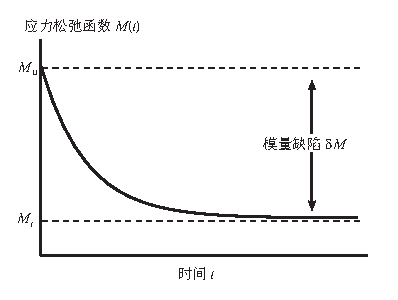
\includegraphics{../figures/chap06/fig01.eps}
\end{center}
\caption[relaxation]{
非弹性介质的应力松弛函数~$M(t)$~从~$t=0$~的未松弛值~$M_{\rm u}$~单调地递减到~$t=\infty$~的已松弛值~$M_{\rm r}$。
}
\end{figure}
\begin{figure}
\begin{center}
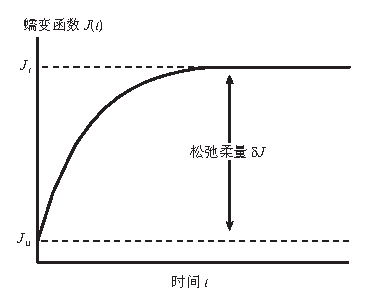
\includegraphics{../figures/chap06/fig02.eps}
\end{center}
\caption[creep]{
蠕变函数~$J(t)$~从~$t=0$~的未松弛值~$J_{\rm u}$~单调递增到~$t=\infty$~的已松弛值~$J_{\rm r}$。
}
\end{figure}
\eq
\delta M=M_{\rm u}-M_{\rm r},\qquad\delta J=J_{\rm r}-J_{\rm u}
\en
分别叫做{\em 模量缺陷\/}和{\em 柔量松弛\/}。
\index{modulus defect}%
\index{compliance!relaxation of}%
\index{relaxation of the compliance}%

在上述讨论中,我们已经将~$t=0$~时刻非零的瞬时平衡响应和~$t=\infty$~时有限的平衡响应视为是理所当然的,因而有
\eq
\label{6.inequal}
0 < M_{\rm r} \leq M_{\rm u} < \infty,\qquad
0 < J_{\rm u} \leq J_{\rm r} < \infty.
\en
在第~6.1.4~节和第~6.1.11~节我们将会看到,这两个假设并不是完全必要的,但它们简化了后续大部分的理论推演。满足~(\ref{6.inequal})~式的介质被称为是{\em 非弹性\/}的。
\index{anelasticity}%
它们有别于更一般的{\em 粘弹性\/}介质,
\index{viscoelasticity}%
因为粘弹性介质可能会有~$M_{\rm r}=1/J_{\rm r}=0$~或~$M_{\rm u}=1/J_{\rm u}=\infty$。

了解所有时间为正~$0\leq t\leq \infty$~的应力松弛函数~$M(t)$~的也意味着了解了蠕变函数~$J(t)$,反之亦然。这两个函数之间的隐含关系可以通过在~(\ref{6.Boltzmann4})~中令~$\sigma(t)=H(t)$~而得到。要注意,~$\varepsilon(t)=J(t)$~在$t=0$~时刻跃变到~$J_{\rm u}$,因而我们有
%%%
\eq
\label{6.MJrel}
1=J_{\rm u}M(t)+\int_0^tM(t-t')\dot{J}(t')\,dt'.
\en
也可以在~(\ref{6.Boltzmann5})~中令~$\varepsilon(t)=H(t)$,或对~(\ref{6.MJrel})~做分部积分,可以得到
%%%
\eq
\label{6.MJrel2}
1=M_{\rm u}J(t)+\int_0^tJ(t-t')\dot{M}(t')\,dt'.
\en
还可以根据下面的关系式,利用~$M(t)$~迭代来获得~$J(t)$,反之亦然。
\eq
\label{6.MJrel3}
t=\int_0^tJ(t')M(t-t')\,dt'=\int_0^tM(t')J(t-t')\,dt'.
\en
将~(\ref{6.MJrel3})~对时间求导,可以证明它与公式~(\ref{6.MJrel})--(\ref{6.MJrel2})~是等价的。将~$M(t-t')=M(t)-[M(t)-M(t-t')]$~这一简单等式代入~(\ref{6.MJrel}),并对含~$M(t)$~的项进行积分,得到
\eq
\label{6.MJrel4}
M(t)J(t)=1+\int_0^t[M(t)-M(t-t')]\dot{J}(t')\,dt'.
\en
实验室测量发现~$M(t)$~和~$J(t)$~这两个函数是单调的;因此,(\ref{6.MJrel4})~中的被积函数总是负的,以至于
\eq
\label{6.inequal3}
M(t)J(t)\leq 1.
\en
我们已经看到,对于~$t=0$~和~$t=\infty$,(\ref{6.inequal3})~中的等式成立;在第~\ref{6.sec.approx}~节中我们则会看到更为普遍的关系是近似相等。
\index{creep function|)}%
\index{stress relaxation function|)}%

%\subsection{Harmonic variations}
\subsection{谐波变化}

到目前为止我们考虑的都是对单位阶跃应力或应变的瞬时响应。我们现在来考虑以谐波形式变化的应力和应变
\eq
\label{6.sigharm}
\sigma(t)=\Re{\rm e}_{\,}[\sigma(\nu)\exp(i\nu t)],\qquad
\varepsilon(t)=\Re{\rm e}_{\,}[\varepsilon(\nu)\exp(i\nu t)].
\en
响应的线性特性确保了若~$\varepsilon(t)$~为~(\ref{6.sigharm})~的形式,则
~$\sigma(t)$~也是,反之亦然。将表达式~(\ref{6.sigharm})~代入玻尔兹曼叠加原理~(\ref{6.Boltzmann4})--(\ref{6.Boltzmann5}),我们发现复数振幅~$\sigma(\nu)$~和~$\varepsilon(\nu)$~之间有如下关系
\eq
\sigma(\nu)=M(\nu)\varepsilon(\nu),\qquad\varepsilon(\nu)=J(\nu)\sigma(\nu),
\en
其中
\eq
\label{6.compM}
M(\nu)=i\nu\int_0^{\infty}M(t)\exp(-i\nu t)\,dt,
\en
\eq
\label{6.compJ}
J(\nu)=i\nu\int_0^{\infty}J(t)\exp(-i\nu t)\,dt.
\en
{\em 复数模量\/}~$M(\nu)$~与{\em 复数柔量\/}~$J(\nu)$~显然是相互关联的:
\index{modulus!complex}%
\index{complex modulus}%
\index{compliance!complex}%
\index{complex compliance}%
\eq
\label{6.MJeq1}
M(\nu)J(\nu)=1.
\en
$M(\nu)$~和~$J(\nu)$~两者都是{\em 解析\/}函数,且在复数频率的{\em 下半\/}平面~($\Im{\rm m}_{\,}\nu\leq 0$)~满足
\eq
\label{6.MJsymms}
M(-\nu^*)=M^*(\nu),\qquad J(-\nu^*)=J^*(\nu)
\en
在频率很低时,应力和应变之间由已松弛的模量和柔量相连:
\eq
\lim_{\nu\rightarrow 0}M(\nu)=
\lim_{\nu\rightarrow 0}1/\!J(\nu)=M_{\rm r}=1/\!J_{\rm r}.
\en
相反,在频率很高时,它们之间由未松弛的模量与柔量相连:
\eq
\lim_{\nu\rightarrow\infty}M(\nu)=
\lim_{\nu\rightarrow\infty}1/\!J(\nu)=M_{\rm u}=1/\!J_{\rm u}.
\en

我们习惯上将实轴上的复数模量和柔量分解为实部和虚部:
\eq
\label{6.MJreim}
M(\omega)=M_1(\omega)+iM_2(\omega),\qquad J(\omega)=J_1(\omega)-iJ_2(\omega).
\en
$M_1(\omega)$、$M_2(\omega)$、$J_1(\omega)$~和~$J_2(\omega)$~可以用~$M(t)$~和~$J(t)$~以显式写为
\eq
M_1(\omega)=\omega\int_0^{\infty}M(t)\sin\omega t\,dt,
\en
\eq
M_2(\omega)=\omega\int_0^{\infty}M(t)\cos\omega t\,dt,
\en
\eq
J_1(\omega)=\omega\int_0^{\infty}J(t)\sin\omega t\,dt,
\en
\eq
J_2(\omega)=-\omega\int_0^{\infty}J(t)\cos\omega t\,dt.
\en
实部模量和柔量均为频率的偶函数,而虚部模量和柔量则均为频率的奇函数:
\eq
\label{6.Msymm}
M_1(-\omega)=M_1(\omega),\qquad M_2(-\omega)=-M_2(\omega),
\en
\eq
\label{6.Jsymm}
J_1(-\omega)=J_1(\omega),\qquad J_2(-\omega)=-J_2(\omega).
\en
(\ref{6.MJreim})~中符号的选择确保了当~$\omega > 0$~时,$M_1(\omega)$、$M_2(\omega)$、$J_1(\omega)$~和~$J_2(\omega)$~这四个函数均为正。

%\subsection{Springs and dashpots}
\subsection{弹簧和阻尼器}
\index{spring|(}%
\index{dashpot|(}%

许多简单的非弹性和粘弹性介质都可以用由线性的弹性弹簧和粘性阻尼器所构成的“拼装玩具”式的网络来模拟或形象化。
\index{tinker-toy}%
组成网络的元件可以有串联或并联的组合形式;这种复合参数力学类比物可以根据几个简单的规则来分析:
\begin{enumerate}
\item 
每个弹簧的本构关系为~$\sigma=M\varepsilon$~或~$\varepsilon=J\sigma$,其中~$M$~为弹性模量,$J=1/M$~为柔量。
\item 
每个阻尼器的本构关系为~$\sigma=\eta\dot{\varepsilon}$,其中~$\eta$~为粘度。
\item 
两个串联的元件应力相等,应变相加,即~$\sigma=\sigma_1=\sigma_2$,$\varepsilon=\varepsilon_1+\varepsilon_2$。
\item 
两个并联的元件应力相加,应变相等,即~$\sigma=\sigma_1+\sigma_2$~和~$\varepsilon=\varepsilon_1=\varepsilon_2$。
\end{enumerate}
每一个由串联或并联的线性弹簧和阻尼器所组成的复合体都相当于一个具有如下形式的{\em 微分本构关系\/}的粘弹性介质:
\index{constitutive relation!differential}%
\index{differential constitutive relation}%
\eq \label{6.diffconst}
a_0\sigma+a_1\dot{\sigma}+a_2\ddot{\sigma}+\cdots=
b_0\varepsilon+b_1\dot{\varepsilon}+b_2\ddot{\varepsilon}+\cdots,
\en
其中~$a_0, a_1, a_2, \ldots$~和~$b_0, b_1, b_2, \ldots$~为实常数。相应的复数模量和柔量是有理多项式:
\eq \label{6.ratpoly}
M(\nu)=\frac{1}{J(\nu)}=
\frac{b_0+b_1(i\nu)+b_2(i\nu)^2+\cdots}
{a_0+a_1(i\nu)+a_2(i\nu)^2+\cdots}.
\en
将上述规则应用于网络结构图,便可确定~$a_0, a_1, a_2, \ldots$~和~$b_0, b_1, b_2, \ldots$~这些系数,这与用基尔霍夫定律确定复合参数电路的整体特性是一样的。基于该做法,\textcite{bland60}~对线性粘弹性理论做了系统性推导。
\index{spring|)}%
\index{dashpot|)}%

%\subsection{Maxwell and Kelvin-Voigt solids}
\subsection{麦克斯韦固体与~Kelvin-Voigt~固体}
\index{Maxwell solid|(}%
\index{Kelvin-Voigt solid|(}%

\begin{figure}[!b]
\begin{center}
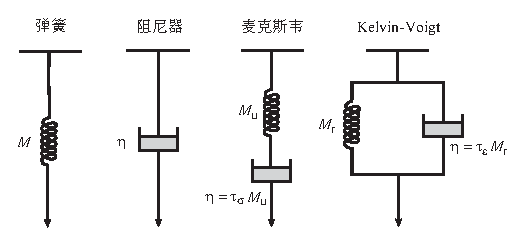
\includegraphics{../figures/chap06/fig03.eps}
\end{center}
\caption[4 networks]{
({\em 从左到右\/})弹簧、阻尼器、麦克斯韦和~Kelvin-Voigt~固体示意图。每个网络都在顶部固定。应力松弛函数~$M(t)$~和蠕变函数~$J(t)$~分别为对作用在箭头处的单位阶跃应变和应力的响应。
}
\end{figure}
这种拼装玩具介质中最简单的是由弹簧和阻尼器串联而成的{\em 麦克斯韦固体\/},以及由弹簧和阻尼器并联而成的{\em Kelvin-Voigt\/}固体。将组成的元件如图~6.3~一样标记,并对应力和应变根据前述规则建立相加或相等的关系,我们得到了这两个单一弹簧加阻尼器固体的微分本构关系
\eq \label{6.MaxKel}
\underbrace{\sigma+\tau_{\sigma}\dot{\sigma}=
\tau_{\sigma}M_{\rm u}\dot{\varepsilon}}_
{\mbox{\rm\scriptsize 麦克斯韦}},
\qquad
\underbrace{\sigma=M_{\rm r}(\varepsilon+
\tau_{\varepsilon}\dot{\varepsilon})}
_{\mbox{\rm\scriptsize Kelvin-Voigt}}.
\en
在~(\ref{6.MaxKel})~式中分别令~$\varepsilon=H(t)$~和~$\sigma=H(t)$,可以得到麦克斯韦与~Kelvin-Voigt~固体的应力松弛函数~$M(t)$~和蠕变函数~$J(t)$。表~6.2~列出了这些函数以及其复数模量~$M(\nu)$~和柔量~$J(\nu)$。
\begin{table}
\centering
\begin{tabular}{|c|c|c|} \hline
&& \\
特性 & 麦克斯韦固体 & Kelvin-Voigt~固体 \\
&& \\ \hline
&& \\
$M(t)$  & $M_{\rm u}\exp(-t/\tau_{\sigma})$
& $M_{\rm r}[\tau_{\varepsilon}\delta(t)+H(t)]$ \\
&& \\
$J(t)$ & $J_{\rm u}[H(t)+t/\tau_{\sigma}]$
& $J_{\rm r}[1-\exp(-t/\tau_{\varepsilon})]$ \\
&& \\ \hline
&& \\
$M(\nu)$ & $M_{\rm u}(i\nu\tau_{\sigma})(1+i\nu\tau_{\sigma})^{-1}$ &
$M_{\rm r}(1+i\nu\tau_{\varepsilon})$ \\
&& \\
$J(\nu)$ & $J_{\rm u}(i\nu\tau_{\sigma})^{-1}(1+i\nu\tau_{\sigma})$ &
$J_{\rm r}(1+i\nu\tau_{\varepsilon})^{-1}$ \\
&& \\ \hline
\end{tabular}
\caption[M&Jdefns]{
两个单一的弹簧加上阻尼器所组成的复合固体的时间域({\em 上\/})和频率域({\em 下\/})特性。
}
\end{table}
$\tau_{\sigma}=\eta/M_{\rm u}$~和~$\tau_{\varepsilon}=\eta/M_{\rm r}$~这两个量分别称为应力和应变{\em 松弛时间\/};
\index{relaxation time!stress}%
\index{relaxation time!strain}%
\index{stress relaxation time}%
\index{strain relaxation time}%
$M_{\rm u}\exp(-t/\tau_{\sigma})$~的指数衰减特性和~$J_{\rm r}[1-\exp(-t/\tau_{\varepsilon})]$~的指数增长特性是这一名称的来源。这两种双元件介质在~(\ref{6.inequal})的意义上都不是非弹性的:麦克斯韦固体在阶跃应力作用下会永远蠕变下去,即$J_{\rm r}=1/M_{\rm r}=\infty$,而~Kelvin-Voigt~固体的瞬时弹性响应是奇异的,即$M_{\rm u}=1/J_{\rm u}=\infty$。
\index{Maxwell solid|)}%
\index{Kelvin-Voigt solid|)}%

%\subsection{Standard linear solid}
\subsection{标准线性固体}
\index{standard linear solid|(}%

\begin{figure}[!b]
\begin{center}
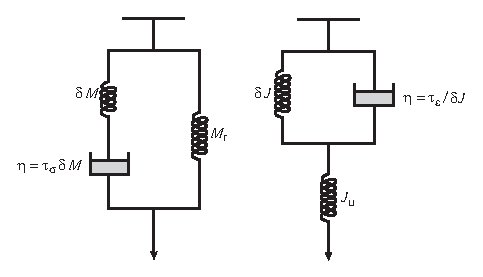
\includegraphics{../figures/chap06/fig04.eps}
\end{center}
\caption[SLS networks]{
等价的标准线性固体的三元件图像表示。({\em 左\/})~麦克斯韦固体和弹簧的并联。({\em 右\/})~Kelvin-Voigt~固体和弹簧的串联。
}
\end{figure}
能满足所有非弹性约束条件的介质最简单的例子是所谓的{\em 标准线性固体\/}。它可以想象成是麦克斯韦固体与弹簧的并联,也可以是~Kelvin-Voigt~固体与弹簧的串联,如图~6.4所示。利用应力和应变的相加和相等规则,我们发现这两种等价的三元件网络的微分本构关系可以写为:
\eq
\label{6.SLS}
\dot{\sigma}+\tau_{\sigma}^{-1}\sigma=M_{\rm u}(\dot{\varepsilon}
+\tau_{\varepsilon}^{-1}\varepsilon),
\en
其中
\eq
\label{6.SLS2}
\delta M/M_{\rm u}=\delta J/J_{\rm r}=1-\tau_{\sigma}/\tau_{\varepsilon}.
\en
与(\ref{6.SLS})~式相应的应力松弛和蠕变函数均为指数形式,但具有不同的衰减与增长时间:
\eq
\label{6.SLS3}
M(t)=M_{\rm u}-\delta M[1-\exp(-t/\tau_{\sigma})],
\en
\eq
\label{6.SLS4}
J(t)=J_{\rm u}+\delta J[1-\exp(-t/\tau_{\varepsilon})].
\en
在~(\ref{6.SLS2})~中我们看到,应力和应变松弛时间之间必须满足~$\tau_{\sigma}\leq\tau_{\varepsilon}$。

\begin{figure}
\begin{center}
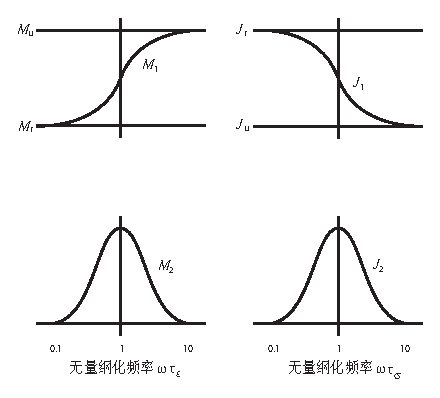
\includegraphics{../figures/chap06/fig05.eps}
\end{center}
\caption[SLS M&J]{
({\em 左\/})标准线性固体的实部模量~$M_1(\omega)$~和虚部模量~$M_2(\omega)$~随频率的变化。({\em 右\/})实部柔量~$J_1(\omega)$~和虚部柔量~$J_2(\omega)$~随频率的变化。注意频率轴为对数。
}
\end{figure}
从~(\ref{6.compM})--(\ref{6.compJ})~或是图~6.4~的频率域分析,我们可以得到标准线性固体的复数模量和柔量
\eq
\label{6.SLS5}
M(\nu)=M_{\rm u}-\delta M(1+i\nu\tau_{\sigma})^{-1},
\en
\eq
\label{6.SLS6}
J(\nu)=J_{\rm u}+\delta J(1+i\nu\tau_{\varepsilon})^{-1}.
\en
值得注意的是,公式~(\ref{6.SLS5})~和~(\ref{6.SLS6})~分别有虚数的简单极点~$\nu=i/\tau_{\sigma}$~和~$\nu=i/\tau_{\varepsilon}$。这是一般非弹性现象的体现——$M(\nu)$~和~$J(\nu)$~的解析延拓会在复数频率的{\em 上半\/}平面($\Im{\rm m}_{\,}\nu > 0$)出现奇点。

在频率实轴上的实部和虚部的模量和柔量为:
\eq
\label{6.Debye}
M_1(\omega)=M_{\rm u}-\frac{\delta M}{1+\omega^2\tau^2_{\sigma}},\qquad
M_2(\omega)=\frac{\omega\tau_{\sigma}\,\delta M}
{1+\omega^2\tau^2_{\sigma}},
\en
\eq
\label{6.Debye4}
J_1(\omega)=J_{\rm u}+\frac{\delta J}{1+\omega^2\tau^2_{\varepsilon}},\qquad
J_2(\omega)=\frac{\omega\tau_{\varepsilon}\,\delta J}
{1+\omega^2\tau^2_{\varepsilon}}.
\en
$M_2(\omega)$~和~$J_2(\omega)$~两者均有所谓{\em 德拜松弛尖峰\/}的形状,峰顶位于
~$\omega\tau=1$,其中~$\tau$~为~$\tau_{\sigma}$~或~$\tau_{\varepsilon}$。
\index{Debye relaxation peak}%
\index{relaxation peak}%
在~$1/10\leq\omega\tau\leq 10$~这一频段之外,虚部模量和柔量相对不重要,如图~6.5~所示。在~$1/10\leq\omega\tau\leq 10$~这一相同的频段内,实部模量$M_1(\omega)$~从~$M_{\rm r}$~增加为~$M_{\rm u}$,相应的柔量~$J_1(\omega)$~从~$J_{\rm r}$~减小为~$J_{\rm u}$。
在这一非弹性频带内的{\em 频散\/}被称为{\em 正常频散\/}。
\index{dispersion!anelastic}%
\index{anelastic dispersion}%
\index{normal dispersion}%
\index{dispersion!normal}%
\index{standard linear solid|)}%

%\subsection{Energy dissipation and \textbf{\textit{Q}}}
\subsection{能量耗散与\textbf{\textit{Q}}}
\index{energy dissipation|(}%
\index{dissipation|(}%
\index{Q@{\em Q}|(}%
\index{quality factor|(}%

在以实频率~$\omega$~做受迫振荡的一个谐波周期内,应力~$\sigma(t)=\Re{\rm e \,}[\sigma(\omega)\exp(i\omega t)]$~和应变~$\varepsilon(t)=\Re{\rm e \,}[\varepsilon(\omega)\exp(i\omega t)]$~的变化遵循一条椭圆形滞后回线,如图~6.6~所示。
\index{hysteresis}%
在一个完整的振荡周期内,单位体积中为克服内摩擦所做的功是滞后回线的面积,可以很容易证明该面积为
\eq
\oint\dot{E}\,dt=\oint\sigma\dot{\varepsilon}\,dt
=\pi M_2(\omega)_{\,}|\varepsilon(\omega)|^2=
\pi J_2(\omega)_{\,}|\sigma(\omega)|^2.
\en
\begin{figure}[!t]
\begin{center}
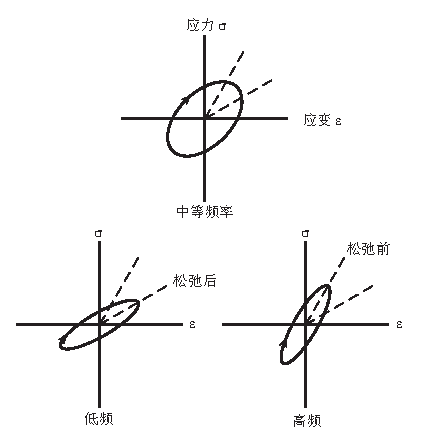
\includegraphics{../figures/chap06/fig06.eps}
\end{center}
\caption[hysteresis]{
受迫振荡的一个谐波周期内应力随应变变化的轨迹。图中所有虚线均表示已松弛和未松弛的纯弹性行为。({\em 上\/})中段频率的应力-应变滞后回线是准圆形的。({\em 下\/})低频和高频的滞后回线则表现出高度的椭圆形;其响应分别为近乎已松弛的~$\sigma\approx M_{\rm r}\varepsilon$和近乎未松弛的~$\sigma\approx M_{\rm u}\varepsilon$。
}
\end{figure}
因此,虚部模量~$M_2(\omega)$~和柔量~$J_2(\omega)$~提供了因非弹性造成的能量的体耗散率的一种度量;能量在物质内部以热的形式耗散。

依照~\textcite{oconnell&budiansky78},非弹性介质的固有品质因子~$Q(\omega)$~的定义为
\index{quality factor!intrinsic}%
\index{intrinsic Q@intrinsic {\em Q}}%
\index{Q@{\em Q}!intrinsic}%
\eq
\label{6.Qdef}
Q(\omega)=\frac{M_1(\omega)}{M_2(\omega)}
=\frac{J_1(\omega)}{J_2(\omega)}.
\en
将复数模量和柔量写成极坐标形式
\eq
M(\omega)=|M(\omega)|\exp[i\phi(\omega)],\qquad
J(\omega)=|J(\omega)|\exp[-i\phi(\omega)],
\en
我们得到品质因子倒数:
\eq
Q^{-1}(\omega)=\tan\phi(\omega).
\en
角度~$\phi(\omega)$~是在谐波滞后回线中应力落后于应变的{\em 相位滞后\/}。
\index{phase lag}%
\index{hysteresis}%

与{\em 耗散的\/}能量相反,在一般非弹性或粘弹性介质中,{\em 储存的\/}弹性能量是一个模糊的概念;
\index{energy!stored}%
\index{stored energy}%
\index{energy!dissipated}%
\index{dissipated energy}%
然而,对于麦克斯韦、~Kelvin-Voigt~或标准线性固体,以及所有其它流变性可以用线性弹簧和阻尼器网络来模拟的介质而言,它可以清楚地定义。\textcite{bland60}~证明,在以实频率~$\omega$~做简谐振荡的一个周期中,这种网络中的一个弹簧所储存的弹性能密度为
\eqa
\label{6.Bland}
\lefteqn{E=\fourth M_1(\omega)_{\,}|\varepsilon(\omega)|^2} \nonumber \\
&&\qquad\mbox{}+\fourth\Re{\rm e\,}\{[M(\omega)-\omega\p_{\omega}M(\omega)]
\varepsilon^2(\omega)\exp(2i\omega t)\} \nonumber \\
&&\mbox{}\!\!\!\!\!\!\!
=\fourth J_1(\omega)_{\,}|\sigma(\omega)|^2 \nonumber \\
&&\qquad\mbox{}+\fourth\Re{\rm e\,}\{[J(\omega)+\omega\p_{\omega}J(\omega)]
\sigma^2(\omega)\exp(2i\omega t)\}.
\ena
与纯弹性一样,瞬时能量密度~$E$~包含一个常数项和一个正比于~$\exp(2i\omega t)$~的项,后者在一个完整的振荡周期内均值为零。因此,固有品质因子具有一个能量的解释——~$4\pi Q^{-1}(\omega)$~是{\em 一个周期内的平均能量耗散比率\/}:
\eq
\label{6.Qinter}
4\pi Q^{-1}=\frac{1}{\langle E_{\,}\rangle}\oint\dot{E}\,dt,
\en
其中
\eq
\langle E_{\,}\rangle =\frac{\omega}{2\pi}\oint E\,dt.
\en
如同~\textcite{oconnell&budiansky78}~所言,“令人费解 \ldots 却又不容置疑的是”非弹性介质中储存的能量不仅依赖于复数模量或柔量在所关注频率的值,还依赖于它们对频率的导数~$\p_{\omega}M(\omega)$~和~$\p_{\omega}J(\omega)$。这便排除了任何以{\em 最大\/}储存能量来简单解释品质因子的可能性。正如我们之前提到的,(\ref{6.Qinter})~这一解释仅适用于可被线弹性弹簧和阻尼器网络模拟的物质。此外,它也仅适用于实数频率为~$\omega$~的纯正弦或余弦的振荡;这种谐波变化通常是用来在实验室中使用谐振仪器来测量~$Q(\omega)$,但在地球上它们却永远不可能自然产生。由地震所激发的自由振荡以~$\exp(i\omega t)$~的方式振荡,但也会在破裂终止后以~$\exp(-\gamma t)$~的
形式随时间衰减。在第~6.1.13~节中我们将看到,
与振荡的时间尺度相比,衰减的时间尺度更为缓慢,即$\gamma\ll\omega$,因而测量地球的固有衰减是有意义的。

将~(\ref{6.Debye})--(\ref{6.Debye4})~两式代入定义式~(\ref{6.Qdef}),并重新组合各项,我们发现标准线性固体的品质因子倒数具有德拜尖峰的形式,其顶点位置为应力和应变松弛时间的几何平均:
\eq
Q^{-1}(\omega)=\frac{\delta M}{\sqrt{M_{\rm u}M_{\rm r}}}
\left(\frac{\omega\overline{\tau}}{1+\omega^2\overline{\tau}^2}\right),
\en
其中~$\overline{\tau}=\sqrt{\tau_{\sigma}\tau_{\varepsilon}}$。这种介质中的耗散在非弹性频带~$1/10\leq\omega\overline{\tau}\leq 10$~以外可忽略不计。
\index{energy dissipation|)}%
\index{dissipation|)}%
\index{Q@{\em Q}|)}%
\index{quality factor|)}%

\renewcommand{\thesubsection}{$\!\!\!\raise1.3ex\hbox{$\star$}\!\!$
\arabic{chapter}.\arabic{section}.\arabic{subsection}}
%\subsection{Kramers-Kronig relations}
\subsection{~Kramers-Kronig~关系}
\index{Kramers-Kronig relations|(}%
\renewcommand{\thesubsection}{\arabic{chapter}.\arabic{section}.\arabic{subsection}}

时间域响应所具有的因果特性导致了在频率域中实部模量~$M_1(\omega)$和虚部模量~$M_2(\omega)$~之间的一个重要关系。要推导这一关系,我们考虑一个有如下性质的复函数~$f(\nu)$:
\begin{enumerate}
\item  
$f(\nu)$~在下半平面$\Im{\rm m}_{\,}\nu\leq 0$是解析函数, \vspace{-2.8 mm}
\item  
当$\nu\rightarrow\infty$~时,$f(\nu)\rightarrow 0$。
\end{enumerate}
第一个性质与柯西定理共同确保这一函数满足
\eq
\label{6.Cauchy}
\oint_C\frac{f(\nu)}{\nu-\omega}\,d\nu=0,
\en
其中~$\omega$~为任意实数,$C$~为积分路径,如图~6.7~所示。
\begin{figure}[!b]
\begin{center}
%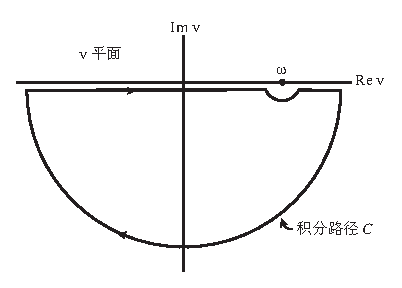
\includegraphics{../figures/chap06/fig07.eps}
\end{center}
\caption[KK contour]{
推导~Kramers-Kronig~关系式~(\ref{6.KK1})--(\ref{6.KK4})~时所使用的积分路径~$C$。
}
\end{figure}
基于第二个性质,在~$\nu\rightarrow\infty$~这一极限下,来自大的半圆弧的贡献为零,因而可以将~(\ref{6.Cauchy})~写为
\eq
\label{6.Cauchy2}
\lim_{\varepsilon\rightarrow 0}\int_{C_{\varepsilon}}
\frac{f(\nu)}{\nu-\omega}\,d\nu
+\lim_{\varepsilon\rightarrow 0}\left(\int_{-\infty}^{-\varepsilon}\!+\!
\int_{\varepsilon}^{\infty}\right)\frac{f(\omega')}{\omega'-\omega}\,d\omega'=0,
\en
其中~$C_{\varepsilon}$~为小的半圆弧,它将点~$\omega$~排除在积分路径之外,$\omega'$~是实的积分哑变量。将~$\nu=\omega+\varepsilon\hspace{0.1 mm}e^{i\theta}$~代入,我们得到~(\ref{6.Cauchy2})~左边的第一个积分项为:
\eq
\label{6.firstint}
\lim_{\varepsilon\rightarrow 0}\int_{C_{\varepsilon}}
\frac{f(\nu)}{\nu-\omega}\,d\nu=\lim_{\varepsilon\rightarrow 0}
i\int_{\pi}^{\textcolor{red}2\pi} f(\omega+\varepsilon\hspace{0.1 mm}e^{i\theta})\,d\theta
=\textcolor{red}{+}i\pi f(\omega).
\en
第二项则定义了一个广义积分的{\em 柯西主值\/},我们之后用一个特殊符号来表示:
\index{Cauchy principal value}%
\index{principal value}%
\eq
\label{6.PVdef}
\pvint_{\!\!-\infty}^{\,\,\infty}
\frac{f(\omega')}{\omega'-\omega}\,d\omega'=
\lim_{\varepsilon\rightarrow 0}\left(\int_{-\infty}^{-\varepsilon}\!+\!
\int_{\varepsilon}^{\infty}\right)\frac{f(\omega')}{\omega'-\omega}\,d\omega'.
\en
合并~(\ref{6.firstint})~和~(\ref{6.PVdef})~两式,我们发现在整个实轴上~$f(\omega)$~必须满足
\eq
\label{6.KKrel}
f(\omega)=\frac{\textcolor{red}{-}1}{i\pi}\pvint_{\!\!-\infty}^{\,\,\infty}
\frac{f(\omega')}{\omega'-\omega}\,d\omega'.
\en

对于任何满足~(\ref{6.inequal})~条件的非弹性固体,$M(\nu)-M_{\rm u}$~和~$J(\nu)-J_{\rm u}$~均具有~$f(\nu)$~所必要的两个性质。
将~$f(\omega)=M(\omega)-M_{\rm u}$~和~$f(\omega)=J(\omega)-J_{\rm u}$~代入~(\ref{6.KKrel}),并令实部和虚部分别相等,我们会得到
\eq
\label{6.KK1}
M_1(\omega)-M_{\rm u}=\frac{\textcolor{red}{-}1}{\pi}\pvint_{\!\!-\infty}^{\,\,\infty}
\frac{M_2(\omega')}{\omega'-\omega}\,d\omega',
\en
\eq
\label{6.KK2}
M_2(\omega)=\textcolor{red}{+}\frac{1}{\pi}\pvint_{\!\!-\infty}^{\,\,\infty}
\frac{M_1(\omega')-M_{\rm u}}{\omega'-\omega}\,d\omega',
\en
\eq
\label{6.KK3}
J_1(\omega)-J_{\rm u}=\frac{1}{\pi}\pvint_{\!\!-\infty}^{\,\,\infty}
\frac{J_2(\omega')}{\omega'-\omega}\,d\omega',
\en
\eq
\label{6.KK4}
J_2(\omega)=-\frac{1}{\pi}\pvint_{\!\!-\infty}^{\,\,\infty}
\frac{J_1(\omega')-J_{\rm u}}{\omega'-\omega}\,d\omega'.
\en
$M_1(\omega)-M_{\rm u}$~和~$M_2(\omega)$~两者互为彼此的{\em 希尔伯特变换\/},$J_1(\omega)-J_u$~和~$J_2(\omega)$~两者也是如此。
\index{Hilbert transform}%
公式~(\ref{6.KK1})--(\ref{6.KK2})~和~(\ref{6.KK3})--(\ref{6.KK4})~被称为~Kramers-Kronig~关系,它们最初是在介电松弛的研究中引入的。
\index{Kramers-Kronig relations}%
值得注意的是,即便有限的平衡响应不存在,即~$M_{\rm r}=0$,但只要~$M_{\rm u}<\infty$,模量之间的关系~(\ref{6.KK1})--(\ref{6.KK2})~依然成立。同样的,即使瞬时弹性响应不存在,即~$J_{\rm u}=0$,但只要~$J_{\rm r}<\infty$,柔量之间的关系~(\ref{6.KK3})--(\ref{6.KK4})~也依然成立。只有对于满足条件~(\ref{6.inequal})~的非弹性固体,上述两对关系才会同时成立。

利用~(\ref{6.Msymm})~和~(\ref{6.Jsymm})~中的奇偶对称性,我们可以将~Kramers-Kronig~关系改写为另一种形式:
\eq
\label{6.KK5}
M_1(\omega)-M_{\rm u}=\frac{\textcolor{red}{-}2}{\pi}\pvint_{\!\!0}^{\,\,\infty}
\frac{\omega'M_2(\omega')}{(\omega'+\omega)(\omega'-\omega)}\,d\omega',
\en
\eq
\label{6.KK6}
M_2(\omega)=\textcolor{red}{+}\frac{2}{\pi}\pvint_{\!\!0}^{\,\,\infty}
\frac{\omega'[M_1(\omega')-M_{\rm u}]}{(\omega'+\omega)(\omega'-\omega)}
\,d\omega',
\en
\eq
\label{6.KK7}
J_1(\omega)-J_{\rm u}=\frac{2}{\pi}\pvint_{\!\!0}^{\,\,\infty}
\frac{\omega'J_2(\omega')}{(\omega'+\omega)(\omega'-\omega)}\,d\omega',
\en
\eq
\label{6.KK8}
J_2(\omega)=-\frac{2}{\pi}\pvint_{\!\!0}^{\,\,\infty}
\frac{\omega'[J_1(\omega')-J_{\rm u}]}{(\omega'+\omega)(\omega'-\omega)}
\,d\omega'.
\en
由~(\ref{6.KK5})--(\ref{6.KK8})~可知,了解所有频率为正~$0<\omega<\infty$~的~$M_2(\omega)$~和~$J_2(\omega)$~也意味了解了~$M_1(\omega)-M_{\rm u}$~和~$J_1(\omega)-J_{\rm u}$~,反之亦然。
\index{Kramers-Kronig relations|)}%

%\subsection{Relaxation and retardation spectrum}
\subsection{松弛谱与迟滞谱}
\index{relaxation spectrum|(}%
\index{spectrum!relaxation|(}%
\index{spectrum!retardation|(}%
\index{retardation spectrum|(}%

从观测发现,地球的固有品质因子~$Q(\omega)$~在~0.3~mHz~到~1~Hz~这一频段内大致与频率无关。因此,全球地震学对~$Q$~为常数的物质有特别感兴趣。该物质的一个有效的现象学模型可以通过考虑具有松弛时间连续谱的标准线性固体的叠加来建立。

将~(\ref{6.SLS3})--(\ref{6.SLS4})~拓展,我们将应力松弛和蠕变函数写为
\eq
\label{6.Mband}
M(t)=M_{\rm u}-\int_0^{\infty}\tau^{-1}Y(\tau)[1-\exp(-t/\tau)]\,d\tau,
\en
\eq
\label{6.Jband}
J(t)=J_{\rm u}+\int_0^{\infty}\tau^{-1}X(\tau)[1-\exp(-t/\tau)]\,d\tau.
\en
复数模量和柔量~(\ref{6.SLS5})--(\ref{6.SLS6})~同样可以拓展为
\eq
\label{6.Mband2}
M(\nu)=M_{\rm u}-\int_0^{\infty}\tau^{-1}Y(\tau)(1+i\nu\tau)^{-1}\,d\tau,
\en
\eq
\label{6.Jband2}
J(\nu)=J_{\rm u}+\int_0^{\infty}\tau^{-1}X(\tau)(1+i\nu\tau)^{-1}\,d\tau.
\en
对于实频率~$\omega$,(\ref{6.Mband2})--(\ref{6.Jband2})~式的实部和虚部为
\eq
\label{6.band1}
M_1(\omega)=M_{\rm u}-\int_0^{\infty}
\frac{Y(\tau)}{1+\omega^2\tau^2}\,\frac{d\tau}{\tau},
\en
\eq
\label{6.band2}
M_2(\omega)=\int_0^{\infty}Y(\tau)\,
\frac{\omega\tau}
{1+\omega^2\tau^2}\,\frac{d\tau}{\tau},
\en
\eq
\label{6.band3}
J_1(\omega)=J_{\rm u}+\int_0^{\infty}
\frac{X(\tau)}{1+\omega^2\tau^2}\,\frac{d\tau}{\tau},
\en
\eq
\label{6.band4}
J_2(\omega)=\int_0^{\infty}X(\tau)\,
\frac{\omega\tau}
{1+\omega^2\tau^2}\,\frac{d\tau}{\tau}.
\en
$Y(\tau)$~和~$X(\tau)$~分别被称为{\em 松弛谱和迟滞谱\/},并满足
\index{relaxation spectrum}%
\index{retardation spectrum}%
\index{spectrum!relaxation}%
\index{spectrum!retardation}%
\eq
\label{6.delMint}
\delta M=\int_0^{\infty}\tau^{-1}Y(\tau)\,d\tau,\qquad
\delta J=\int_0^{\infty}\tau^{-1}X(\tau)\,d\tau.
\en
很显然$\tau^{-1}Y(\tau)$~是在松弛时间为~$\tau$~和~$\tau+d\tau$~之间,物质内部因非弹性过程所造成的模量缺陷~$\delta M$~的一种度量,而~$\tau^{-1}X(\tau)$~则对应于柔量松弛~$\delta J$~的一种度量。被积函数中的“额外的”因子~$\tau^{-1}$~是出于习惯。一种物质的非弹性性质可以用~(\ref{6.band1})--(\ref{6.band4})~来表述,则该物质被称为{\em 吸收带固体\/}。
\index{absorption-band solid}%
\index{relaxation spectrum|)}%
\index{spectrum!relaxation|)}%
\index{spectrum!retardation|)}%
\index{retardation spectrum|)}%
 
%\subsection{Approximate relations}
\subsection{近似关系}
\label{6.sec.approx}

Kramers-Kroni~关系~(\ref{6.KK5})--(\ref{6.KK8})~使得实部模量~$M_1(\omega)$~和虚部模量~$M_2(\omega)$~之间或实部柔量~$J_1(\omega)$~和虚部柔量~$J_2(\omega)$~之间不存在任何精确的局地关系。然而,当松弛和迟滞谱~$Y(\tau)$~和~$X(\tau)$~在一个很宽的松弛时间范围内缓慢变化时,则存在一个简单的近似关系。

正如之前所见,德拜尖峰函数~$\omega\tau/(1+\omega^2\tau^2)$~在~$1/10\leq\omega\tau\leq 10$~这两个量级以外可以忽略不计。如果松弛谱~$Y(\tau)$~在此范围内没有显著变化,在公式~(\ref{6.band2})~中我们可以将其移到积分外面,而得到如下近似
\eq
\label{6.approx1}
M_2(\omega)\approx\omega Y(1/\omega)\int_0^{\infty}
\frac{d\tau}{1+\omega^2\tau^2}=\half\pi Y(1/\omega).
\en
实部模量~(\ref{6.band1})~对频率的偏导数同样可近似为
\eqa \label{6.approx2} \lefteqn{
\frac{\p M_1(\omega)}{\p\omega}=
2\omega\int_0^{\infty}\frac{\tau Y(\tau)}
{(1+\omega^2\tau^2)^2}\,d\tau} \nonumber \\
&&\mbox{}\hspace{5.9 mm}\approx \textcolor{red}{2\omega^{-1}Y(1/\omega)\int_0^{\infty}
\frac{\omega\tau\,d(\omega\tau)}{(1+\omega^2\tau^2)^2}}
=\omega^{-1}Y(1/\omega).
\ena
(\ref{6.band1})~式中的函数~$1/(1+\omega^2\tau^2)$~具有阶梯状特征,在同一~$1/10\leq\omega\tau\leq 10$~范围内从~1~降到~0。将该阶梯状函数在~$\omega\tau=1$~处近似为一个陡峭的阶梯,可以得到:
\eq
\label{6.M1approx}
M_1(\omega)\approx M_{\rm u}-\int_0^{1/\omega}
\tau^{-1}Y(\tau)\,d\tau.
\en
对(\ref{6.M1approx})~式的微分又得到~(\ref{6.approx2})~式,因此这两个近似是自洽的。对比~(\ref{6.approx1})~和~(\ref{6.approx2})~这两个结果,可以得到所寻求的实部和虚部模量之间的关系:
\eq
\label{6.diffapprox}
\frac{\p M_1(\omega)}{\p\omega}\approx\frac{2M_2(\omega)}{\pi\omega},
\en
或等价于
\eq
\label{6.approx3}
\frac{\p\ln M_1(\omega)}{\p\ln \omega}\approx
\frac{2}{\pi Q(\omega)},
\en
这里我们使用了定义式~(\ref{6.Qdef})。近似式~(\ref{6.approx3})~将实部模量的对数频散~$\p\ln M_1(\omega)/_{\!}\p\ln\omega$~与位于相同频率~$\omega$~处的品质因子~$Q(\omega)$~联系起来。当~$Q(\omega)$不随频率存在剧烈变化时,上式是一个有用的近似。

将(\ref{6.approx3})~积分我们得到
\eq
\label{6.Mapprox}
\frac{M_1(\omega)}{M_1(\omega_0)}\approx 1+
\frac{2}{\pi}\int_{\omega_0}^{\omega}\frac{d\omega'}
{\omega'Q(\omega')},
\en
其中~$\omega$~和~$\omega_0$~均假设为正,且~$Q(\omega)\gg 1$。实部柔量显然也有类似的结果,但会是一个负号,即
\eq
\label{6.Japprox}
\frac{J_1(\omega)}{J_1(\omega_0)}\approx 1-
\frac{2}{\pi}\int_{\omega_0}^{\omega}\frac{d\omega'}
{\omega'Q(\omega')}.
\en
在~$\omega$~和~$\omega_0$~的范围内具有~$Q(\omega)\approx Q$~的{\em 常数~$Q$~物质\/}会表现出{\em 对数频散\/}
\index{Q@{\em Q}!constant}%
\index{quality factor!constant}%
\index{constant-$Q$ material}%
\index{dispersion!logarithmic}%
\index{logarithmic dispersion}%
\eq
\label{6.MCONSTQ}
\frac{M_1(\omega)}{M_1(\omega_0)}\approx1+\frac{2}{\pi Q}\ln
\left(\frac{\omega}{\omega_0}\right),
\en
\eq
\label{6.JCONSTQ}
\frac{J_1(\omega)}{J_1(\omega_0)}\approx1-\frac{2}{\pi Q}\ln
\left(\frac{\omega}{\omega_0}\right).
\en
比较~(\ref{6.Mapprox})~和~(\ref{6.Japprox})~这两个公式,我们发现当~$Q(\om)\gg 1$~时,实部模量和柔量可近似互为倒数,即
\eq
\label{6.M1J1approx}
M_1(\omega)J_1(\omega)\approx 1.
\en
(\ref{6.M1J1approx})~式是对精确的模量-柔量关系~$M_1(\omega)J_1(\omega)+M_2(\omega)J_2(\omega)=1$~的一个近似,后者可由~(\ref{6.MJeq1})~式得到。

对于应力松弛函数~$M(t)$~和蠕变函数~$J(t)$~也可以推导出类似的近似关系。(\ref{6.Mband})~式中的~$1-\exp(-t/\tau)$~也是一个阶梯状函数,在~$1/10\leq t/\tau\leq 10$~范围内从~0~增加到~1。将其以一个具有在~$t/\tau =1$~处的陡峭阶梯替换,我们得到
\eq
M(t)\approx M_{\rm u}-\int_0^t\tau^{-1}Y(\tau)\,d\tau.
\en
将此式与~(\ref{6.M1approx})~式对比,我们看到应力松弛函数~$M(t)$~与实部模量~$M_1(\omega)$~之间存在一个简单关系:
\eq
\label{6.Mtapprox}
M(t)\approx\left.M_1(\omega)\right|_{\omega=1/t}.
\en
蠕变函数~$J(t)$~和实部柔量~$J_1(\omega)$~也同样满足:
\eq
\label{6.Jtapprox}
J(t)\approx\left.J_1(\omega)\right|_{\omega=1/t}.
\en
将~(\ref{6.M1J1approx})~和~(\ref{6.Mtapprox})--(\ref{6.Jtapprox})~这三个近似相结合,可以得到最后一个有益的关系式,即
\eq
\label{6.MtJtapprox}
M(t)J(t)\approx 1.
\en
将此结果与严格的关系式~(\ref{6.inequal3})~对比也很有意思。

\renewcommand{\thesubsection}{$\!\!\!\raise1.3ex\hbox{$\star$}\!\!$
\arabic{chapter}.\arabic{section}.\arabic{subsection}}
%\subsection{Constant-{\textbf{\textit{Q}}} absorption-band model}
\subsection{常数~{\textbf{\textit{Q}}}~吸收带模型}
\index{absorption-band model|(}%
\renewcommand{\thesubsection}{\arabic{chapter}.\arabic{section}.\arabic{subsection}}

遵循~Liu,Anderson~与~Kanamori~(\citeyear{liu&al76})~和~Kanamori~与~Anderson~(\citeyear{kanamori&anderson77})~的方法,我们可以通过选取一个矩形的松弛谱或迟滞谱来构建一个特定频段~$1/\tau_{\rm M}\ll\omega\ll 1/\tau_{\rm m}$~内的常数~$Q$~模型:
\eq
\label{6.Ybox}
Y(\tau)=\left\{\begin{array}{ll}
\delta\hspace{-0.2 mm}M/_{\!}\ln(\tau_{\rm M}/_{\!}\tau_{\rm m})
& \mbox{当 $\tau_{\rm m}\leq\tau\leq\tau_{\rm M}$时} \\
$0$ & \mbox{其它情形,}
\end{array}\right.
\en
\eq
\label{6.Xbox}
X(\tau)=\left\{\begin{array}{ll}
\delta\hspace{-0.2 mm}J/_{\!}\ln(\tau_{\rm M}/_{\!}\tau_{\rm m})
& \mbox{当 $\tau_{\rm m}\leq\tau\leq\tau_{\rm M}$时} \\
$0$ & \mbox{其它情形.}
\end{array}\right.
\en
将~(\ref{6.Ybox})--(\ref{6.Xbox})~代入~(\ref{6.Mband2})--(\ref{6.Jband2})~并进行积分,我们得到
\eq
\label{6.MBAND}
M(\nu)=M_{\rm r}+\left[\frac{\delta\hspace{-0.2 mm}M}
{\ln(\tau_{\rm M}/\tau_{\rm m})}\right]
\ln\left(\frac{i\nu\tau_{\rm M}+1}
{i\nu\tau_{\rm m}+1}\right),
\en
\eq
\label{6.JBAND}
J(\nu)=J_{\rm r}-\left[\frac{\delta\hspace{-0.2 mm}J}
{\ln(\tau_{\rm M}/\tau_{\rm m})}\right]
\ln\left(\frac{i\nu\tau_{\rm M}+1}
{i\nu\tau_{\rm m}+1}\right),
\en
其中$M_{\rm r}=M_{\rm u}-\delta\hspace{-0.2 mm}M$和$J_{\rm r}=J_{\rm u}+\delta\hspace{-0.2 mm}J$仍遵循之前的定义。复数模量~(\ref{6.MBAND})~和柔量~(\ref{6.JBAND})~除了在正虚轴上的~$\nu=i/_{\!}\tau_{\rm M}$~和~$\nu=i/_{\!}\tau_{\rm m}$~两点之间它们呈现{\em 对数分支切割\/},在其它任何地方都是解析的。
\index{logarithmic branch cut}% 
\index{branch cut!logarithmic}% 
对于实频率~$\omega$,(\ref{6.MBAND})~和~(\ref{6.JBAND})~的实部与虚部分别为
\eq
\label{6.MBAND1}
M_1(\omega)=M_{\rm r}+\half\left[\frac{\delta\hspace{-0.2 mm}M}
{\ln(\tau_{\rm M}/_{\!}\tau_{\rm m})}\right]
\ln\left(\frac{1+\omega^2\tau_{\rm M}^2}
{1+\omega^2\tau_{\rm m}^2}\right),
\en
\eq
\label{6.MBAND2}
M_2(\omega)=\left[\frac{\delta\hspace{-0.2 mm}M}
{\ln(\tau_{\rm M}/_{\!}\tau_{\rm m})}\right]
\arctan\left[\frac{\omega(\tau_{\rm M}-\tau_{\rm m})}
{1+\omega^2\tau_{\rm m}\tau_{\rm M}}\right]
\en
和
\eq
\label{6.JBAND1}
J_1(\omega)=J_{\rm r}-\half\left[\frac{\delta\hspace{-0.2 mm}J}
{\ln(\tau_{\rm M}/_{\!}\tau_{\rm m})}\right]
\ln\left(\frac{1+\omega^2\tau_{\rm M}^2}
{1+\omega^2\tau_{\rm m}^2}\right),
\en
\eq
\label{6.JBAND2}
J_2(\omega)=\left[\frac{\delta\hspace{-0.2 mm}J}
{\ln(\tau_{\rm M}/_{\!}\tau_{\rm m})}\right]
\arctan\left[\frac{\omega(\tau_{\rm M}-\tau_{\rm m})}
{1+\omega^2\tau_{\rm m}\tau_{\rm M}}\right].
\en

(\ref{6.MBAND1})--(\ref{6.MBAND2})~和~(\ref{6.JBAND1})--(\ref{6.JBAND2})~这两组四参数表达式只有在宽带、弱衰减介质满足以下条件时是等价的
\eq \label{6.liu}
\tau_{\rm m}\ll\tau_{\rm M},\qquad
\delta\hspace{-0.2 mm}M\ll M_{\rm u},M_{\rm r},\qquad
\delta\hspace{-0.2 mm}J\ll J_{\rm u},J_{\rm r}.
\en
如图~6.8~所示,该介质的品质因子~$Q(\omega)=M_1(\omega)/M_2(\omega)=J_1(\om)/J_2(\om)$~在~$1/\tau_{\rm M}\ll\omega\ll 1/\tau_{\rm m}$~频段内基本上与频率无关。
\begin{figure}[!b]
\begin{center}
\scalebox{0.95}{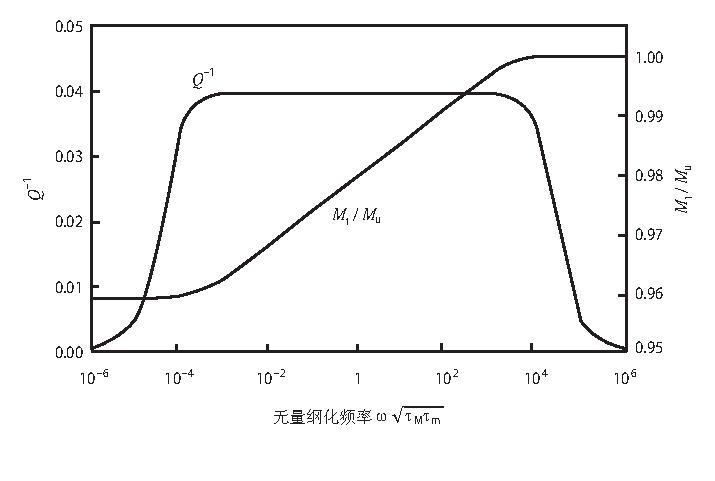
\includegraphics{../figures/chap06/fig08.eps}}
\end{center}
\caption[absorption band]{
典型的吸收带固体的无量纲实部模量~$M_1(\omega)/M_{\rm u}$~和品质因子倒数~$Q^{-1}(\omega)$~随频率的变化。此处频带高低边界的频率比是~$\tau_{\rm M}/\tau_{\rm m}=10^7$,在吸收带内品质因子是~$Q=250$;而无量纲模量缺陷~$\delta\hspace{-0.2 mm}M/M_{\rm u}$~为~4.1~$\%$。
}
\end{figure}
在{\em 常数~Q~吸收带\/}内,其数值可以由以下任何一个等价关系给定
\eq
\frac{2}{\pi Q}\ln\left(\frac{\tau_{\rm M}}{\tau_{\rm m}}\right)
\approx\frac{\delta\hspace{-0.2 mm}M}{M_{\rm u}}
\approx\frac{\delta\hspace{-0.2 mm}M}{M_{\rm r}}
\approx\frac{\delta\hspace{-0.2 mm}J}{J_{\rm u}}
\approx\frac{\delta\hspace{-0.2 mm}J}{\textcolor{red}{J}_{\rm r}}.
\en
(\ref{6.liu})~中的条件确保了~$Q\gg 1$。实部模量~(\ref{6.MBAND1})~和柔量~(\ref{6.JBAND1})~在常数~$Q$~频带内可很好地近似为
\eq
\label{6.DISPER}
M_1(\omega)\approx M_{\rm u}\left[1+\frac{2}{\pi Q}
\ln(\omega\tau_{\rm m})\right]
\approx M_{\rm r}\left[1+\frac{2}{\pi Q}
\ln(\omega\tau_{\rm M})\right],
\en
\eq \label{6.DISPERJ}
J_1(\omega)\approx J_{\rm u}\left[1-\frac{2}{\pi Q}
\ln(\omega\tau_{\rm m})\right]
\approx J_{\rm r}\left[1-\frac{2}{\pi Q}
\ln(\omega\tau_{\rm M})\right].
\en
值得注意的是,$M_1(\om)J_1(\om)\approx 1$,与~(\ref{6.M1J1approx})~式相符。将~(\ref{6.Ybox})--(\ref{6.Xbox})~两个谱代入表达式~(\ref{6.Mband})--(\ref{6.Jband}),可以得到与模量~(\ref{6.MBAND})~和柔量~(\ref{6.JBAND})~相对应的应力松弛函数~$M(t)$~和蠕变函数~$J(t)$。这便使得一对指数积分在~$\tau_{\rm m}\ll t\ll\tau_{\rm M}$~的范围内可以近似为
\eq \label{6.Lomnitz}
M(t)\approx M_{\rm u}\left[1-\frac{2}{\pi Q}
\ln\left(\frac{t}{\tau_{\rm m}}\right)\right]
\approx M_{\rm r}\left[1-\frac{2}{\pi Q}
\ln\left(\frac{t}{\tau_{\rm M}}\right)\right],
\en
\eq \label{6.Lomnitz2}
J(t)\approx J_{\rm u}\left[1+\frac{2}{\pi Q}
\ln\left(\frac{t}{\tau_{\rm m}}\right)\right]
\approx J_{\rm r}\left[1+\frac{2}{\pi Q}
\ln\left(\frac{t}{\tau_{\rm M}}\right)\right],
\en
正如预期的,(\ref{6.Lomnitz})--(\ref{6.Lomnitz2})~符合~(\ref{6.Mtapprox})--(\ref{6.MtJtapprox})~这两个近似关系。Lomnitz在早期实验室岩石形变观测中已经注意到(\ref{6.Lomnitz2})~形式的对数行为(\citeyear{lomnitz56}; \citeyear{lomnitz57}),因而在地球物理学界该对数行为也被称为{\em Lomnitz~蠕变定律\/}。
\index{Lomnitz's law of creep}%
\index{absorption-band model|)}%


\renewcommand{\thesubsection}{$\!\!\!\raise1.3ex\hbox{$\star$}\!\!$
\arabic{chapter}.\arabic{section}.\arabic{subsection}}
%\subsection{Strictly constant \textbf{\textit{Q}} model}
\subsection{严格的常数~\textbf{\textit{Q}}~模型}
\index{Q@{\em Q}!constant|(}%
\index{quality factor!constant|(}%
\index{constant-$Q$ material|(}%
\label{6.sec.Kjart}
\renewcommand{\thesubsection}{\arabic{chapter}.\arabic{section}.\arabic{subsection}}

在频率~$0<\omega<\infty$~范围上,任何非弹性物质的~$Q(\omega)$~都不会是严格的常数;然而,如果我们放宽非弹性约束~(\ref{6.inequal}),这种介质就并不难找。遵循~\textcite{kjartansson79},我们考虑下面的蠕变函数:
\eq
\label{6.KjartJ}
J(t)=\frac{(\omega_0t)^q}{M_{0\,}\Gamma(1+q)}H(t),
\en
其中~$\omega_0$,$M_0$~和~$q$~均为正常数,$\Gamma(1+q)$~表示伽马函数。相应于(\ref{6.KjartJ})~的复数柔量可以很容易地用~(\ref{6.compJ})~得到
\eq
\label{6.KjartJ2}
J(\nu)
=\frac{1}{M_0}\left(\frac{i\nu}
{\omega_0}\right)^{\!-q}.
\en
复数模量必须是~(\ref{6.KjartJ2})~的倒数,即
\eq
\label{6.KjcompM}
M(\nu)=
M_0\left(\frac{i\nu}{\omega_0}\right)^q.
\en
对~(\ref{6.KjcompM})~式做傅里叶逆变换,我们得到应力松弛函数:
\eq
\label{6.KjartM}
M(t)=\frac{M_0(\omega_0t)^{-q}}{\Gamma(1-q)}H(t).
\en
由~(\ref{6.KjartJ})--(\ref{6.KjartM})~这四个关系所表征的粘弹性物质满足~$J_{\rm u}=1/M_{\rm u}=0$~和~$J_{\rm r}=1/M_{\rm r}=\infty$;因此,它既无瞬时弹性响应也没有长期平衡响应。常数~$M_0$~可以被视为绝对模量~$|M(\omega)|$~在基准实频率~$\omega=\omega_0$~处的值。

复数模量~(\ref{6.KjcompM})~和柔量~(\ref{6.KjartJ2})~的实部和虚部分别为:
\eq
M_1(\omega)=M_0\left|\frac{\omega}{\omega_0}\right|
^q\cos\left(\half\pi q_{\,}{\rm sgn}_{\,}\omega\right),
\en
\eq
M_2(\omega)=M_0\left|\frac{\omega}{\omega_0}\right|
^q\sin\left(\half\pi q_{\,}{\rm sgn}_{\,}\omega\right),
\en
\eq
J_1(\omega)=\frac{1}{M_0}\left|\frac{\omega}{\omega_0}\right|
^{-q}\cos\left(\half\pi q_{\,}{\rm sgn}_{\,}\omega\right),
\en
\eq
J_2(\omega)=\frac{1}{M_0}\left|\frac{\omega}{\omega_0}\right|
^{-q}\sin\left(\half\pi q_{\,}{\rm sgn}_{\,}\omega\right),
\en
其中~$\omega$~假定为实数,${\rm sgn}_{\,}\omega$~为符号函数:
\eq
{\rm sgn}_{\,}\omega=\left\{\begin{array}{ll}
+1 & \mbox{当 $\omega > 0$时} \\
-1 & \mbox{当 $\omega < 0$时.}
\end{array}\right.
\en
正如之前许诺的,品质因子~$Q(\omega)=M_1(\omega)/M_2(\omega)
=J_1(\omega)/J_2(\omega)$~完全与频率无关:
\eq
Q(\omega)=Q\,{\rm sgn}_{\,}\omega\quad
\mbox{其中}\quad Q^{-1}=\tan(\half\pi q).
\en
在~$\omega=0$~处的不连续确保了~$Q(\omega)$~具有必要的奇对称性~$Q(-\omega)=-Q(\omega)$。正的实频率~$\omega > 0$~的频散关系为
\eq
\label{6.DISPER2}
\frac{M_1(\omega)}{M_1(\omega_0)}=
\left(\frac{\omega}{\omega_0}\right)^q\approx
1+\frac{2}{\pi Q}\ln\left(\frac{\omega}{\omega_0}\right),
\en
\eq \label{6.DISPER2J}
\frac{J_1(\omega)}{J_1(\omega_0)}=
\left(\frac{\omega}{\omega_0}\right)^{\!-q}\approx
1-\frac{2}{\pi Q}\ln\left(\frac{\omega}{\omega_0}\right),
\en
两式中最后面的近似等式在~$Q\gg 1$~时都是成立的。

(\ref{6.MCONSTQ})--(\ref{6.JCONSTQ})、(\ref{6.DISPER})--(\ref{6.DISPERJ})~和~(\ref{6.DISPER2})--(\ref{6.DISPER2J})~这三个独立的表达式尽管是在迥异的假设下所推导出来的,但它们的一致性显示了该基本结果的可靠性。频散的对数特性对相比较的两个频率范围以外的非弹性行为的细节不敏感;唯一重要的条件是在这两个频率范围之内~$Q(\omega)$~与频率无关。
\index{Q@{\em Q}!constant|)}%
\index{quality factor!constant|)}%
\index{constant-$Q$ material|)}%

\renewcommand{\thesubsection}{$\!\!\!\raise1.3ex\hbox{$\star$}\!\!$
\arabic{chapter}.\arabic{section}.\arabic{subsection}}
%\subsection{Power-law \textbf{\textit{Q}} model}
\subsection{幂律~\textbf{\textit{Q}}~模型}
\index{Q@{\em Q}!power-law|(}%
\index{quality factor!power-law|(}%
\index{power-law $Q$ model|(}%
\renewcommand{\thesubsection}{\arabic{chapter}.\arabic{section}.\arabic{subsection}}

遵循~\textcite{anderson&minster79},我们可以通过考虑如下形式的松弛谱或迟滞谱来得到频率依赖性较弱的~$Q(\om)$
\eq
\label{6.YAndMin}
Y(\tau)=\left\{\begin{array}{ll}
\alpha\,(\delta\hspace{-0.2 mm}M)\tau^{\alpha}/
(\tau_{\rm M}^{\alpha}-\tau_{\rm m}^{\alpha})
& \mbox{当 $\tau_{\rm m}\leq\tau\leq\tau_{\rm M}$时} \\
$0$ & \mbox{其它情形,}
\end{array}\right.
\en
\eq
\label{6.XAndMin}
X(\tau)=\left\{\begin{array}{ll}
\alpha\,(\delta\hspace{-0.2 mm}J)\tau^{\alpha}/
(\tau_{\rm M}^{\alpha}-\tau_{\rm m}^{\alpha})
& \mbox{当 $\tau_{\rm m}\leq\tau\leq\tau_{\rm M}$时} \\
$0$ & \mbox{其它情形,}
\end{array}\right.
\en
其中~$0 < \alpha \ll 1$。我们将~(\ref{6.YAndMin})--(\ref{6.XAndMin})~代入公式~(\ref{6.band1})--(\ref{6.band4}),并利用~(\ref{6.liu})~中的近似来计算吸收带~$1/\tau_{\rm M}\ll\omega\ll 1/\tau_{\rm m}$~内的积分。所得到的品质因子~$Q(\omega)=M_1(\omega)/M_2(\omega)=J_1(\omega)/J_2(\omega)$~表现出随频率的幂律式变化:
\eq
\label{6.powerQ}
Q(\omega)\approx Q_0(\omega/\omega_0)^{\alpha},
\en
其中~$Q_0=Q(\omega_0)$。与形如~(\ref{6.powerQ})~的衰减定律相应的实部模量和柔量为:
\eq
\label{6.AndMin}
\frac{M_1(\omega)}{M_1(\omega_0)}\approx
1+\frac{2}{\alpha\pi Q_0}
\left[1-\left(\frac{\omega}
{\omega_0}\right)^{\!-\alpha}\right],
\en
\eq
\label{6.AndMin2}
\frac{J_1(\omega)}{J_1(\omega_0)}\approx
1-\frac{2}{\alpha\pi Q_0}
\left[1-\left(\frac{\omega}
{\omega_0}\right)^{\!-\alpha}\right].
\en
正如所预期的,在与频率无关的极限~$\alpha\rightarrow 0$~下,公式~(\ref{6.AndMin})--(\ref{6.AndMin2})~退化为对数型的常数~$Q$~结果,并且有形如~(\ref{6.powerQ})~的较弱的频率依赖性时,它们与一般频散规律~(\ref{6.Mapprox})--(\ref{6.Japprox})~是一致的。
\index{Q@{\em Q}!power-law|)}%
\index{quality factor!power-law|)}%
\index{power-law $Q$ model|)}%

\renewcommand{\thesubsection}{$\!\!\!\raise1.3ex\hbox{$\star$}\!\!$
\arabic{chapter}.\arabic{section}.\arabic{subsection}}
%\subsection{Behavior near the real frequency axis}
\subsection{实频轴附近的表现}
\renewcommand{\thesubsection}{\arabic{chapter}.\arabic{section}.\arabic{subsection}}

一个自由衰减的简正模式在其复频率~$\nu=\omega+i\gamma$~处“看到”地球的非弹性模量和柔量。由于衰减时间比振荡的本征周期长很多,人们的兴趣在于探讨~$M(\nu)$~和~$J(\nu)$~在正实频轴附近的表现。遵循~\textcite{oconnell&budiansky78},我们将模量以其实部和虚部写为如下形式
\eqa
\label{6.Mneareal}
\lefteqn{M(\omega+i\gamma)=F(\omega,\gamma)+iG(\omega,\gamma)} \\
&&\mbox{}\,\,\,\,\,\,\,\,\,\,\,\,\,\,\,\,
\approx F(\omega,0)+\gamma\p_{\gamma}F(\omega,0)
+i[G(\omega,0)+\gamma\p_{\gamma}G(\omega,0)], \nonumber 
\ena
其中的近似在~$\gamma\ll\omega$~时成立。假设~$M(\omega+i\gamma)$~在实轴附近是解析的,我们可以利用柯西-黎曼方程将~(\ref{6.Mneareal})~写为
\eqa
\label{6.Mneareal2}
\lefteqn{M(\omega+i\gamma)\approx F(\omega,0)-\gamma\p_{\omega}G(\omega,0)
+i[G(\omega,0)+\gamma\p_{\omega}F(\omega,0)]} \nonumber \\
&&\mbox{}\,\,\,\,\,\,\,\,\,\,\,\,\,\,\,\,
= M_1(\omega)-\gamma\p_{\omega}M_2(\omega)
+i[M_2(\omega)+\gamma\p_{\omega}M_1(\omega)].
\ena
将定义式~(\ref{6.Qdef})~和近似式~(\ref{6.diffapprox})~代入~(\ref{6.Mneareal2}),我们得到
\eqa
\label{6.MmodeApprox}
\lefteqn{
M(\omega+i\gamma)\approx M_1(\omega)\{1+Q^{-2}(\omega)
[\gamma\p_{\omega}Q(\omega)-2\gamma/\pi\omega]\}} \nonumber \\
&&\mbox{}\qquad\qquad\qquad
+iM_1(\omega)Q^{-1}(\omega)(1+2\gamma/\pi\omega),
\ena
上式精确到~$Q^{-1}$~和~$\gamma/_{\!}\omega$~的二阶。与其有同样精度的柔量为
\eqa
\label{6.JmodeApprox}
\lefteqn{
J(\omega+i\gamma)\approx J_1(\omega)\{1+Q^{-2}(\omega)
[\gamma\p_{\omega}Q(\omega)-2\gamma/\pi\omega]\}} \nonumber \\
&&\mbox{}\qquad\qquad\qquad
-iJ_1(\omega)Q^{-1}(\omega)(1+2\gamma/\pi\omega).
\ena
再进一步简化,我们可以忽略~(\ref{6.MmodeApprox})--(\ref{6.JmodeApprox})~中的二阶项,将它们以~$Q^{-1}$~和~$\gamma/_{\!}\omega$~的一阶精度写为:
\eq
\label{6.Mmodeapprox}
M(\omega+i\gamma)\approx M_1(\omega)[1+iQ^{-1}(\omega)],
\en
\eq
\label{6.Jmodeapprox}
J(\omega+i\gamma)\approx J_1(\omega)[1-iQ^{-1}(\omega)].
\en
对于地球而言,由于~$Q(\omega)\gg 1$,因而~$\gamma\ll\omega$,一般认为最后两个近似式足以满足地震学的要求。(\ref{6.Mmodeapprox})--(\ref{6.Jmodeapprox})~这两个结果只是表明每一个简正模式是在其振荡的实频率~$\omega$~处“看到”地球的非弹性。这是符合基本的物理直觉的。

%\subsection{Bulk and shear quality factors}
\subsection{体变与剪切品质因子}
\index{Q@{\em Q}!bulk|(}%
\index{Q@{\em Q}!shear|(}%
\index{quality factor!bulk|(}%
\index{bulk quality factor|(}%
\index{shear quality factor|(}%
\index{quality factor!shear|(}%

总而言之,一个各向同性的流体静力学地球模型中,地震能量的耗散可以通过将弹性不可压缩性~$\kappa$~和刚度~$\mu$~用复数的、依赖频率的非弹性参数替换来处理。在这样的地球中,等价于~(\ref{6.Boltzmann})~式的频率域本构关系为
\eqa
\label{6.unoagn}
\lefteqn{
\bT^{\rm L1}(\omega)=\kappa(\omega)
[1+iQ^{-1}_{\kappa}(\omega)]\theta(\omega)\bI} \nonumber \\
&&\mbox{}\qquad\qquad\qquad
+2\mu(\omega)[1+iQ^{-1}_{\mu}(\omega)]\bd(\omega),
\ena
其中,为符号的简洁性起见,我们略去了实部模量~$\kappa(\omega)$~和~$\mu(\omega)$~的下角标~1。$Q_{\kappa}(\omega)$~和~$Q_{\kappa}(\omega)$~分别被称为{\em 体变和剪切品质因子\/}。
\index{Q@{\em Q}!bulk}%
\index{Q@{\em Q}!shear}%

更普遍地,我们可以将任意流体静力学地球模型中的拉格朗日柯西应力增量写为如下形式
\eq
\label{6.Boltzmann2}
\bT^{\rm L1}(\omega)=\bGamma(\omega)\!:\!\beps(\omega),
\en
其中
\eqa
\label{6.Gamdef}
\lefteqn{
\Gamma_{ijkl}(\omega)=\{\kappa(\omega)[1+iQ^{-1}_{\kappa}(\omega)]
-\twothirds\mu(\omega)[1+iQ^{-1}_{\mu}(\omega)]\}_{\,}\delta_{ij\,}\delta_{kl}} \nonumber \\
&&\mbox{}+\mu(\omega)[1+iQ^{-1}_{\mu}(\omega)]_{\,}(\delta_{ik\,}\delta_{jl}
+\delta_{il\,}\delta_{jk})+\gamma_{ijkl},
\ena
并且将任意非流体静力地球模型中的~Piola-Kirchhoff~应力增量写为
\eq
\label{6.Boltzmann3}
\bT^{\rm PK1}(\omega)=\bLambda(\omega)\!:\!\bdel\bs(\omega),
\en
其中
\eqa
\lefteqn{
\label{6.Lamdef}
\Lambda_{ijkl}(\omega)=\{\kappa(\omega)[1+iQ^{-1}_{\kappa}(\omega)]
-\twothirds\mu(\omega)
[1+iQ^{-1}_{\mu}(\omega)]\}_{\,}\delta_{ij\,}\delta_{kl}} \nonumber \\
&&\mbox{}+\mu(\omega)[1+iQ^{-1}_{\mu}(\omega)]_{\,}(\delta_{ik\,}\delta_{jl}
+\delta_{il\,}\delta_{jk})+\gamma_{ijkl} \\
&&\mbox{}+\half(T^{\,0}_{ij\,}\delta_{kl}
+T^{\,0}_{kl\,}\delta_{ij}
+T^{\,0}_{ik\,}\delta_{jl}-T^{\,0}_{jk\,}\delta_{il}
-T^{\,0}_{il\,}\delta_{jk}-T^{\,0}_{jl\,}\delta_{ik}). \nonumber
\ena
(\ref{6.Gamdef})~和~(\ref{6.Lamdef})~中的各向异性张量~$\bgamma$~被认为是完全弹性的;因而~$\bGamma(\omega)$~和~$\bLambda(\omega)$~中仅有不可压缩性~$\kappa(\omega)[1+iQ^{-1}_{\kappa}(\omega)]$~和刚度~$\mu(\omega)[1+iQ^{-1}_{\mu}(\omega)]$的频散项是复数的。(\ref{6.Boltzmann2})~和~(\ref{6.Boltzmann3})~两式与物质参照系无关原理~(\ref{2.last1})--(\ref{2.last2})~一致,这当然是它们必须满足的。
\index{frame indifference}%
我们也可以很容易地建立一个非弹性的完全各向异性理论,其中的~$\bgamma$~换成一个复数的依赖频率的张量~$\bgamma(\om)$;然而,目前没有任何地震学证据显示有建立这种理论的必要性。在~$Q^{-1}_{\kappa}(\omega)$~和~$Q^{-1}_{\mu}(\omega)$~中所体现的地球的各向同性的非弹性,以及在实张量~$\bgamma$~中所体现的弹性的各向异性,两者都很弱;即便是高度受控的实验也仅能对该特性的分布提供相当有限的信息。毫无疑问,尽管各向异性的非弹性会出现在多晶固体中,但它却是“加倍地微弱”。因此,地球的非弹性通常被视为是各向同性的。

在一阶近似下,频率为正~$\omega > 0$~时,(\ref{6.Gamdef})~和~(\ref{6.Lamdef})~中的体变与剪切品质因子可以被看作是不随频率变化的:
\eq
\label{6.conQmukap}
Q_{\kappa}(\omega)\approx Q_{\kappa},\qquad
Q_{\mu}(\omega)\approx Q_{\mu},
\en
此时相应的频散是对数形式的:
\index{logarithmic dispersion}%
\index{dispersion!logarithmic}%
\eq
\label{6.kappadisp}
\frac{\kappa(\omega)}{\kappa(\omega_0)}\approx
1+\frac{2}{\pi Q_{\kappa}}\ln\left(\frac{\omega}{\omega_0}\right),
\en
\eq
\label{6.mudisp}
\frac{\mu(\omega)}{\mu(\omega_0)}\approx
1+\frac{2}{\pi Q_{\mu}}\ln\left(\frac{\omega}{\omega_0}\right).
\en
为简单起见,我们在本书之后的绝大部分的章节中采用常数~$Q$~的对数频散定律~(\ref{6.kappadisp})--(\ref{6.mudisp})。然而在全球地震学所关注的频带内,体变或剪切品质因子的任何微弱的频率依赖性都可以根据需求,以更普遍的近似式~(\ref{6.Mapprox})~或~(\ref{6.AndMin})~加以考虑。
\index{Q@{\em Q}!bulk|)}%
\index{Q@{\em Q}!shear|)}%
\index{quality factor!bulk|)}%
\index{bulk quality factor|)}%
\index{shear quality factor|)}%
\index{quality factor!shear|)}%
\index{anelasticity|)}%

%\section{Non-Rotating Anelastic Earth}
\section{无自转非弹性地球}
\index{Earth model!non-rotating, anelastic|(}%
\label{6.sec.nonrot}

在本节和下一节,我们将展示第~4~章的结果可以推广至非弹性介质。在这些纯形式的讨论中,我们不必将注意力局限于各向同性的常数~$Q$~地球,或者做出任一模式在其振荡的实频率~$\omega$~处“看到”地球的非弹性这一近似。事实上,如果考虑由如下复数的、依赖频率的本构关系所描述的一般非弹性地球模型,在符号表示上会更为简单
\eq \label{6.rewrite}
\bT^{\rm PK1}(\nu)=\bLambda(\nu)\!:\!\bdel\bs(\nu)
\quad\mbox{其中}\quad\bLambda(-\nu^*)=\bLambda^*(\nu).
\en
以下,我们只会偶尔考虑有实际兴趣的特例。同样地,为便于讨论,我们会将无自转地球和自转地球两种情形分开;首先,我们来考虑较为简单的无自转~($\bOmega=\bzero$)~情形。

%\subsection{Duality and biorthonormality}
\subsection{对偶性与双正交归一性}
\index{duality!non-rotating Earth|(}
\index{biorthonormality!non-rotating Earth|(}
\label{6.sec.duality}

要获得无自转非弹性地球的复数本征频率~$\nu$~及其对应的本征函数~$\bs$,需要求解抽象的算子方程
\eq
\label{6.Hsnus}
\sH(\nu)\bs=\nu^2\bs,
\en
其中~$\sH(\nu)$~表示地球模型~$\earth$~中的积分-微分算子,满足
\index{integro-differential operator}%
\index{operator!integro-differential}%
\eq
\label{6.Hnrdef}
\rho^0\sH(\nu)\bs=-\bdel\cdot[\bLambda(\nu)\!:\!\bdel\bs]
+\rho^0\bdel\phi^{\rm E1}+\rho^0\bs\cdot\bdel\bdel\phi^0
\en
以及在~$\p\earth$、$\Sigma_{\rm SS}$~和~$\Sigma_{\rm FS}$~上相应的边界条件。非弹性-引力算子~(\ref{6.Hnrdef})~具有动力学对称性
\eq
\label{6.Hadjsymm}
\sH(-\nu^*)=\sH^*(\nu),
\en
其中~$\rho^0\sH^*(\nu)\bs=-\bdel\cdot[\bLambda^*(\nu)\!:\!\bdel\bs]
+\rho^0\bdel\phi^{\rm E1}+\rho^0\bs\cdot\bdel\bdel\phi^0$。取~(\ref{6.Hsnus})~式的复共轭,并利用~(\ref{6.Hadjsymm})~式,我们可以看到,当且仅当~$\nu$、$\bs$~是无自转非弹性地球的一组本征解时,$-\nu^*$、$\bs^*$~也是无自转非弹性地球的另一组本征解。

在~$\earth$~中,任意两个分段平滑的复函数~$\bs$~和~$\bs'$~的{\em 内积\/}被定义为
\index{inner product!non-rotating Earth}%
\eq
\label{6.inprod}
\langle\bs,\bs'\rangle=\int_{\subearth}\rho^0\bs^*\cdot\bs'\,dV.
\en
借由类似于第~\ref{4.sec.nrHerm}~节中对弹性无自转地球的推论,我们可以利用热力学对称性~$\Lambda_{ijkl}(\nu)=\Lambda_{klij}(\nu)$~来证明
\eq
\label{6.Hermdef}
\langle\bs,\sH(\nu)\bs'\rangle=\langle\sH^*(\nu)\bs,\bs'\rangle
=\langle\bs',\sH^*(\nu)\bs\rangle^*.
\en
因此,$\sH^*(\nu)$~是算子~$\sH(\nu)$~的{\em 厄米特伴随\/}算子。
\index{adjoint operator}%
\index{Hermitian adjoint operator}%
\index{operator!Hermitian adjoint}%
我们可以将~$\bs^*$~视为原来算子~$\sH(-\nu^*)$~的本征征频率为~$-\nu^*$~的本征函数,或者是伴随算子~$\sH^*(\nu)$~的本征征频率为~$\nu$~的本征函数。该算子与其伴随算子通常具有互为复共轭的谱;在当前的情形下,其相应的本征函数之间的关系尤为简单——它们也是彼此的复共轭。

振荡简正模式的{\em 品质因子\/}~$Q$~可以用其实数正本征频率~$\omega=\Re{\rm e}\,\nu$~和衰减率~$\gamma=\Im{\rm m}\,\nu$~定义为
\index{Q@{\em Q}!of a mode}%
\index{quality factor!of a mode}%
\eq
Q^{-1}=2\gamma / \omega.
\en
取~$\sH(\nu)\bs=\nu^2\bs$~与本征函数~$\bs$~的内积的虚部,我们有
\eq \label{6.ReImnu}
2(\Re{\rm e}\,\nu)(\Im{\rm m}\,\nu)
\int_{\subearth}\rho^0\bs^*\cdot\bs\,dV=
\int_{\subearth}\bdel\bs^*\!:\!\Im{\rm m}
\,\bLambda(\nu)\!:\!\bdel\bs\,dV.
\en
对于固有品质因子~$Q_{\kappa}$~和~$Q_{\mu}$~不随频率变化的非弹性各向同性地球,该关系成为
\eq
\label{6.Qmodeqn}
Q^{-1}=\frac{\displaystyle{\int_{\subearth}}[\kappa(\omega)Q_{\kappa}^{-1}
(\bdel\cdot\bs^*)(\bdel\cdot\bs)+2\mu(\omega)Q_{\mu}^{-1}
(\bd^*\!:\!\bd)]\,dV}
{\omega^2\displaystyle{\int_{\subearth}}\rho^0\bs^*\cdot\bs\,dV},
\en
为简便起见,这里我们使用了弱衰减近似~(\ref{6.Mmodeapprox})。体变和剪切品质因子~$Q_{\kappa}$~和~$Q_{\mu}$~的正值性意味着~$Q>0$,这确保了所有的本征频率~$\nu=\omega+i\gamma$~均位于复频率平面的上半平面,也证实了简正模式因非弹性耗散必须随时间{\em 衰减\/}这一物理上显而易见的结果。
\index{decay}%

除了内积~(\ref{6.inprod})~之外,我们也可以方便地将星号去掉,来定义在~$\earth$~中任意两个复函数的第二种双线性积:
\eq
\label{6.dualprod}
[\bs,\bs']=\int_{\subearth}\rho^0\bs\cdot\bs'\,dV.
\en
(\ref{6.Hermdef})~式可以改写为:
\eq
\label{6.Hdualsymm}
[\bs,\sH(\nu)\bs']=[\sH(\nu)\bs,\bs']=[\bs',\sH(\nu)\bs],
\en
因而~$\sH(\nu)$~在这个新定义的积下是{\em 对称的\/}。
\index{symmetric operator}%
\index{operator!symmetric}%
我们将~(\ref{6.dualprod})~称为{\em 对偶积\/};
\index{duality product!non-rotating Earth}%
这一称谓的来源将会在第~6.3.1~节中加以说明。取$\sH(\nu)\bs=\nu^2\bs$~与~$\bs'$~的对偶积可得
\eq
\label{6.dual1}
\nu^2[\bs',\bs]=[\bs',\sH(\nu)\bs],
\en
而取~$\sH(\nu')\bs'=\nu^{\prime 2}\bs'$~与~$\bs$~的对偶积则有
\eq
\label{6.dual2}
\nu^{\prime 2}[\bs,\bs']=[\bs,\sH(\nu')\bs'].
\en
用~(\ref{6.dual1})~式减去~(\ref{6.dual2})~式,并利用对称性~(\ref{6.Hdualsymm}),我们得到
\eq
\label{6.orthog}
[\bs,\bs']-(\nu^2-\nu^{\prime 2})^{-1}
[\bs,\{\sH(\nu)-\sH(\nu')\}\bs']=0
\quad\mbox{当 $\nu\neq\nu'$时}.
\en
(\ref{6.orthog})~式是简正模式正交条件~(\ref{4.NORMAL})~在非弹性情形下的推广。

在目前的情形下,不同的本征频率~$\nu$~和~$\nu'$~所对应的两个本征函数~$\bs$~和~$\bs'$~在~(\ref{6.orthog})~的意义上是正交的这种说法并不精确,因为~$[\bs,\bs']$~并非复数空间内的一个合理内积。实际上,~(\ref{6.orthog})~所表达的是与~$-\nu^*$~和~$\nu'$~相对应的本征函数~$\bs^*$~和~$\bs'$~之间的{\em 双正交性\/}。
\index{biorthogonality!non-rotating Earth}%
当任何本征函数~$\bs$~与其复共轭~$\bs^*$~具有不同的本征频率~$\nu\neq -\nu^*$时,双正交性~(\ref{6.orthog})~成为~(\ref{6.ReImnu})。(\ref{6.orthog})~式左边的量在~$\nu'\rightarrow\nu$~极限下的定义是十分明确的,因此我们可以方便地将本征函数归一化,使得在此极限下有
\index{normalization condition!non-rotating, anelastic Earth}%
\eq
\label{6.normal}
[\bs,\bs]-\half\nu^{-1}[\bs,\p_{\nu}\sH(\nu)\bs]=1.
\en
其优点是,在无频散~$\p_{\nu}\sH(\nu)=0$~时,该式退化为无自转弹性地球上所采用的归一化定义~(\ref{4.ANORMAL})。
\index{duality!non-rotating Earth|)}
\index{biorthonormality!non-rotating Earth|)}

%\subsection{Rayleigh's principle}
\subsection{瑞利原理}
\index{Rayleigh's principle!non-rotating, anelastic Earth|(}%
\label{6.sec.Rayprin}

只要把内积~(\ref{4.inprod})~换为对偶积~(\ref{6.dualprod}),在第~\ref{4.sec.Rayprin}~节中所阐述的各种形式的瑞利原理都仍然成立。将~(\ref{4.firstact})~式推广,我们定义非弹性地球内的{\em 作用量\/}
\index{action}%
\eq
\label{6.firstact}
\sI=\half\nu^2[\bs,\bs]-\half[\bs,\sH(\nu)\bs].
\en
瑞利原理表明,对于任意可容许的变化~$\bdelta\bs$,当且仅当~$\bs$~是非弹性地球的本征频率为~$\nu$~的本征函数时,该复数泛函是稳定的。要验证这一点,我们注意到,当精确到~$\|\bdelta\bs\|$~的一阶时有
\eq
\delta\sI={\rm Re}\,[\bdelta\bs,\nu^2\bs-\sH(\nu)\bs],
\en
这里我们使用了算子~$\sH(\nu)$~的对称性~(\ref{6.Hdualsymm})。显然,对于任意~$\bdelta\bs$,当且仅当~$\sH(\nu)\bs=\nu^2\bs$~时,$\delta \sI$~为零。

作用量~(\ref{6.firstact})~可以用显式写为
\eq
\label{6.action}
\sI=\int_{\subearth}L(\bs,\bdel\bs)\,dV
+\int_{\Sigma_{\rm FS}}L^{\Sigma}(\bs,\bdel^{\Sigma}\bs)\,d\Sigma,
\en
其中
\eqa
\label{6.Lagdef}
\lefteqn{
L=\half[\nu^2\rho^0\bs\cdot\bs-\bdel\bs\!:\!
\bLambda(\nu)\!:\!\bdel\bs} \nonumber \\
&&\mbox{}\qquad\qquad-\rho^0\bs\cdot\bdel\phi^{\rm E1}-\rho^0
\bs\cdot\bdel\bdel\phi^0\cdot\bs],
\ena
\eq
L^{\Sigma}=\half[(\bnh\cdot\bs)\bdel^{\Sigma}\cdot(\varpi^0\bs)
-\varpi^0(\bs\cdot\bdel^{\Sigma}\bs\cdot\bnh)].
\en
我们将~(\ref{6.Lagdef})~式中的欧拉势函数微扰~$\phi^{\rm E1}$~视为由~(\ref{3.phiE1int2})~式给定的~$\bs$~的已知泛函,因此~$\delta\sI=0$~是一个位移变分原理。
\index{variational principle!displacement}%

如同在无自转弹性地球上一样,也有一个位移-势函数变分原理,其中~$\bs$~和~$\phi^{\rm E1}$~是独立变量;
\index{variational principle!displacement-potential}%
该变分原理中修改后的作用量为
\eq
\label{6.modact}
\sI'=\int_{\subspace}L'(\bs,\bdel\bs,\bdel\phi^{\rm E1})\,dV
+\int_{\Sigma_{\rm FS}}L^{\Sigma}(\bs,\bdel^{\Sigma}\bs)\,d\Sigma,
\en
其中
\eqa
\lefteqn{
L'=\half[\nu^2\rho^0\bs\cdot\bs-\bdel\bs\!:\!\bLambda(\nu)\!:\!\bdel\bs
-2\rho^0\bs\cdot\bdel\phi^{\rm E1}} \nonumber \\
&&\mbox{}\qquad-\rho^0
\bs\cdot\bdel\bdel\phi^0\cdot\bs
-(4\pi G)^{-1}\bdel\phi^{\rm E1}\cdot\bdel\phi^{\rm E1}].
\ena
对于每组非弹性本征解~$\nu$、$\bs$、$\phi^{\rm E1}$,两个非弹性作用量的稳定值均为~$\sI=\sI'=0$。
\index{Rayleigh's principle!non-rotating, anelastic Earth|)}%

%\subsection{Green tensor}
\subsection{格林张量}
\index{Green tensor!non-rotating, anelastic Earth|(}%
\index{tensor!Green!non-rotating, anelastic|(}%
\label{6.sec.Green}

在第~\ref{4.sec.nrGreen}~节中,我们直接在时间域中确定了无自转弹性地球的格林张量~$\bG(\bx,\bx';t)$。对于非弹性地球,考虑复频率域中格林张量的傅里叶变换会更加方便
\eq
\bG(\bx,\bx';\nu)=\int_0^{\infty}\bG(\bx,\bx';t)\exp(-i\nu t)\,dt,
\en
对应的逆变换为
\eq
\label{6.invFtrf}
\bG(\bx,\bx';t)=\frac{1}{2\pi}\int_{-\infty}^{\infty}
\bG(\bx,\bx';\nu)\exp(i\nu t)\,d\nu,
\en
其中积分路径是沿着频率实轴,如图~6.9~所示。
\begin{figure}[!b]
\begin{center}
%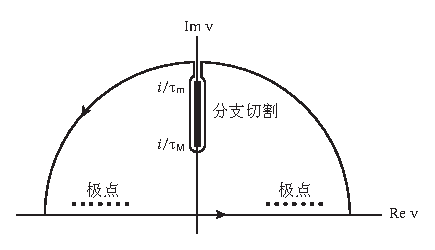
\includegraphics{../figures/chap06/fig09.eps}
\end{center}
\caption[ Green contour]{
计算傅里叶逆变换~(\ref{6.invFtrf})~时所使用的积分路径。当~$t<0$~时,积分路径在下半平面闭合。由于下半平面没有极点或其他奇点,因此${\bf G}
({\bf x},{\bf x}';t)={\bf 0}$。当~$t>0$~时,积分路径在上半平面闭合,如图所示。在此仅考虑复本征频率~$\nu_k$~和~$-\nu_k^*$~处简单极点的留数,并忽略所有被积函数在跨越对数分支切割~$i/\tau_{\rm M}\leq\nu\leq i/\tau_{\rm m}$~时的不连续性,因而推导出~(\ref{6.GREEN})~这一简单的结果。
%%%
}
\end{figure}
要得到频率域格林张量~$\bG(\bx,\bx';\nu)$,我们需要求解
\eq
\label{6.Green1}
\rho^0[-\nu^2\bG+\sH(\nu)\bG]=\bI_{\,}\delta(\bx-\bx').
\en
取~(\ref{6.Green1})~的复共轭,并利用对称性~(\ref{6.Hadjsymm})~式,我们得到
\eq
\label{6.Greensymm}
\bG(\bx,\bx';-\nu^*)=\bG^*(\bx,\bx';\nu).
\en
因此,只要得到右半平面~$\Re{\rm e}_{\,}\nu > 0$~的~$\bG(\bx,\bx';\nu)$~就足够了;在左半平面~$\Re{\rm e}_{\,}\nu < 0$~的值可以用~(\ref{6.Greensymm})~式得到。

我们用~$k$~来标记右半平面上的本征频率~$\nu_k$~及其相应的本征函数~$\bs_k$;左半平面上所对应的本征频率和本征函数则分别为~$-\nu_k^*$~和~$\bs_k^*$。右半平面上本征频率为~$\nu_k\neq\nu_{k'}$~的本征函数的双正交关系~(\ref{6.orthog})~可用显式写为
\index{biorthogonality!non-rotating Earth}%
\eqa
\label{6.orthog2}
\lefteqn{
\int_{\subearth}\rho^0\bs_k\cdot\bs_{k'}\,dV} \nonumber \\
&&\mbox{}-(\nu_k^2-\nu_{k'}^2)^{-1}\int_{\subearth}\beps_k\!:\!
[\bGamma(\nu_k)-\bGamma(\nu_{k'})]\!:\!\beps_{k'}\,dV=0.
\ena
同样地,非弹性归一化条件~(\ref{6.normal})~式可表示为
\index{normalization condition!non-rotating, anelastic Earth}%
\eq
\label{6.normal2}
\int_{\subearth}\rho^0\bs_k\cdot\bs_k\,dV
-\half\nu_k^{-1}\int_{\subearth}\beps_k\!:\!
\p_{\nu}\bGamma(\nu_k)\!:\!\beps_{k}\,dV=1.
\en
出现在~(\ref{6.orthog2})--(\ref{6.normal2})~中的弹性张量是~$\bGamma(\nu)$~而不是~$\bLambda(\nu)$,因为两者之差~$\bLambda(\nu)-\bGamma(\nu)$~仅依赖于初始偏应力~$\btau^0$,所以与频率~$\nu$~无关。我们寻求非齐次方程~(\ref{6.Green1})~如下形式的解
\eq
\label{6.Greensum}
\bG(\bx,\bx';\nu)=\sum_k\bs_k(\bx)\bc_k(\bx';\nu),\quad
\Re{\rm e}_{\,}\nu > 0.
\en
为了得到时间域格林张量~$\bG(\bx,\bx';t)$~正规的简正模式叠加形式,我们做下面两个近似:
\begin{enumerate}
\item 我们忽略{\em 本征频率简并\/}的可能性,并假设右半平面上所有的本征频率都是不同的。
\index{eigenfrequency degeneracy}%
\index{degeneracy}%
\item 我们也忽略{\em 对数分支切割\/}的影响,
\index{logarithmic branch cut}%
\index{branch cut!logarithmic}%
        以及~$\bLambda(\nu)$~在复数频率的上半平面~$\Im{\rm m}_{\,}\nu\geq 0$~中其它任何奇点的影响。因此,所考虑的奇点只有~$\bG(\bx,\bx';\nu)$~在复本征频率~$\nu_k$~和~$-\nu_k^*$~处的{\em 简单极点\/}。
\index{simple pole}%
\index{pole!simple}%
\end{enumerate}
我们利用留数方法来计算~(\ref{6.invFtrf})~中的积分,在上半平面~$t > 0$~将积分路径闭合,以确保无穷远处圆弧的贡献为零。通过引入上述两个近似,我们得到
\eqa
\label{6.CAUCHY}
\lefteqn{
\bG(\bx,\bx';t)=2_{\,}\Re{\rm e}\sum_k\bs_k(\bx)
\left[\lim_{\nu\rightarrow\nu_k}
i(\nu-\nu_k)\bc_k(\bx';\nu)\right]
\exp(i\nu_kt)_{\,}.} \nonumber \\
&&\mbox{}
\ena
(\ref{6.CAUCHY})~中方括号内的量是~$i$~乘以~$\nu=\nu_k$~处简单极点的留数;在对应的~$\nu=-\nu_k^*$~处的极点也已利用对称关系~(\ref{6.Greensymm})~加以考虑。要计算留数,我们将叠加式~(\ref{6.Greensum})~代入~(\ref{6.Green1}),并取其与~$\bs_k$~的对偶积,重组各项后得到
\eqa
\label{6.Greencalc}
\lefteqn{\bc_k(\bx';\nu)=\frac{\bs_k(\bx')}
{[\bs_k,\sH(\nu)\bs_k-\nu^2\bs_k]}} \nonumber \\
&&\mbox{}\qquad\qquad\qquad-\sum_{k'\neq k}
\frac{[\bs_k,\sH(\nu)\bs_{k'}-\nu^2\bs_{k'}]}
{[\bs_k,\sH(\nu)\bs_k-\nu^2\bs_k]}\,\bc_{k'}(\bx';\nu).
\ena
为了便于达到极限,我们在分母中进一步加上~$\sH(\nu_k)\bs_k-\nu_k^2\bs_k=\bzero$,经过一些推导得到
\eqa
\label{6.Greencalc2}
\lefteqn{\lim_{\nu\rightarrow\nu_k}
i(\nu-\nu_k)\bc_k(\bx';\nu)=
\frac{i\bs_k(\bx')}
{[\bs_k,\p_{\nu}\sH(\nu_k)\bs_k]-2\nu_k[\bs_k,\bs_k]}} \nonumber \\
&&\mbox{}\qquad-\sum_{k'\neq k}
\frac{i[\bs_k,\sH(\nu_k)\bs_{k'}-\nu_k^2\bs_{k'}]}
{[\bs_k,\p_{\nu}\sH(\nu_k)\bs_k]-2\nu_k[\bs_k,\bs_k]}\,
\bc_{k'}(\bx';\nu_k).
\ena
因为算子~$\sH(\nu)$~的对称性~(\ref{6.Hdualsymm}),(\ref{6.Greencalc2})~中对~$k'\neq k$~的求和为零:
\eq
[\bs_k,\sH(\nu_k)\bs_{k'}-\nu_k^2\bs_{k'}]=
[\bs_{k'},\sH(\nu_k)\bs_k-\nu_k^2\bs_k]=0.
\en
因此,(\ref{6.CAUCHY})~中的展开系数可以简化为
\eq
\lim_{\nu\rightarrow\nu_k}
i(\nu-\nu_k)\bc_k(\bx';\nu)=
\half(i\nu_k)^{-1}\bs_k(\bx'),
\en
这里我们使用了归一化条件~(\ref{6.normal2})。最终格林张量可以用复本征频率和本征函数表示为
\eq
\label{6.GREEN}
\bG(\bx,\bx';t)=\Re{\rm e}\sum_k(i\nu_k)^{-1}
\bs_k(\bx)\bs_k(\bx')\exp(i\nu_kt).
\en
无自转非弹性地球的平凡模式与相应的无自转弹性地球的模式相同,因为其中的刚体模式不具有形变,而地转模式也均局限于耗散可以被忽略的液态区域~$\earth_{\rm F}$。但由于平凡模式不能被固态地壳或地幔中的地震所激发,我们从~(\ref{6.GREEN})~的简正模式叠加中将其剔除,并将剩下的仅包含地震模式的叠加称为{\em 地震格林张量\/}。值得注意的是~(\ref{6.GREEN})~满足关系
%%%
\eq
\bG(\bx,\bx';t)=\bG^{\rm T}(\bx',\bx;t),
\en
因此,{\em 源点-接收点互易性\/}原理在无自转非弹性地球上仍然成立。
\index{reciprocity}%
\index{Green tensor!non-rotating, anelastic Earth|)}%
\index{tensor!Green!non-rotating, anelastic|)}%
\index{Earth model!non-rotating, anelastic|)}%

\renewcommand{\thesection}{$\!\!\!\raise1.3ex\hbox{$\star$}\!\!$
\arabic{chapter}.\arabic{section}}
%\section{Rotating Anelastic Earth}
\section{自转非弹性地球}
\index{Earth model!rotating, anelastic|(}%
\label{6.sec.rot}
\renewcommand{\thesection}{\arabic{chapter}.\arabic{section}}

\textcite{lognonne91}~首次正确地处理了自转非弹性地球这种一般的情形。在本节中我们简述他们的结果。

\renewcommand{\thesubsection}{$\!\!\!\raise1.3ex\hbox{$\star$}\!\!$
\arabic{chapter}.\arabic{section}.\arabic{subsection}}
%\subsection{Duality and biorthonormality}
\subsection{对偶性和双正交归一性}
\index{duality!rotating Earth|(}%
\index{biorthonormality!rotating Earth|(}%
\label{6.sec.duality2}
\renewcommand{\thesubsection}{\arabic{chapter}.\arabic{section}.\arabic{subsection}}

要得到自转非弹性地球的复本征频率~$\nu$~及其相应的本征函数~$\bs$,我们需求解抽象的算子方程
\eq
\label{6.Hroteqn}
\sH(\nu)\bs+2i\nu_{\,}\bOmega\times\bs=\nu^2\bs.
\en
此处~$\sH(\nu)$~表示考虑离心势函数的修改后的积分-微分算子
\index{integro-differential operator}%
\index{operator!integro-differential}%
\eq
\label{6.Hrotdef}
\rho^0\sH(\nu)\bs=-\bdel\cdot[\bLambda(\nu)\!:\!\bdel\bs]
+\rho^0\bdel\phi^{\rm E1}+\rho^0\bs\cdot\bdel\bdel(\phi^0+\psi),
\en
并满足与其相应的~$\p\earth$、$\Sigma_{\rm SS}$~和~$\Sigma_{\rm FS}$~上的边界条件。弹性张量的对称性~$\bLambda(-\nu^*)=\bLambda^*(\nu)$~确保了
\eq
\label{6.Hadjsymr}
\sH(-\nu^*)=\sH^*(\nu),
\en
其中~$\rho^0\sH^*(\nu)\bs=-\bdel\cdot[\bLambda^*(\nu)\!:\!\bdel\bs]
+\rho^0\bdel\phi^{\rm E1}+\rho^0\bs\cdot\bdel\bdel(\phi^0+\psi)$。取~(\ref{6.Hroteqn})~的复共轭,并利用~(\ref{6.Hadjsymr}),我们发现当且仅当~$\nu$、$\bs$~为一组本征解时,$-\nu^*$、$\bs^*$~也是一组本征解。同无自转非弹性地球的情形一样,在~(\ref{6.inprod})~所定义的内积下,$\sH^*(\nu)$~是~$\sH(\nu)$~的{\em 伴随\/}算子。
\index{adjoint operator}%
\index{operator!adjoint}%

自转方向相反~($\bOmega\rightarrow -\bOmega$)~的逆转地球的本征频率和本征函数也值得关注。
\index{anti-Earth}%
实际地球和逆转地球具有{\em 相同的复本征频率\/}~$\nu$,但相应的本征函数却不同,我们分别表示为~$\bs$~和~$\overline{\bs}$。我们称逆转地球的本征函数~$\overline{\bs}$~为{\em 对偶本征函数\/};
\index{eigenfunction!dual}%
\index{dual eigenfunction}%
要得到对偶本征函数,除了求解方程~(\ref{6.Hroteqn})~之外,我们还需要求解
\eq
\label{6.antiHeqn}
\sH(\nu)\overline{\bs}-2i\nu_{\,}
\bOmega\times\overline{\bs}=\nu^2\overline{\bs},
\en
对称性~(\ref{6.Hadjsymr})~确保了如果~$\nu$、$\overline{\bs}$~为~(\ref{6.antiHeqn})~的一组本征解,则~$-\nu^*$、$\overline{\bs}^{\,\raisebox{-.5ex}{\scriptsize{*}}}$~亦然。

取~(\ref{6.Hrotdef})~式与~$\bs$~的内积的虚部,并利用近似关系~(\ref{6.Mmodeapprox})~和~(\ref{6.Lamdef}),我们得到
\index{Q@{\em Q}!of a mode}%
\index{quality factor!of a mode}%
\eq
\label{6.Qmoderot}
Q^{-1}=\frac{\displaystyle{\int_{\subearth}}[\kappa(\omega)Q_{\kappa}^{-1}
(\bdel\cdot\bs^*)(\bdel\cdot\bs)+2\mu(\omega)Q_{\mu}^{-1}
(\bd^*\!:\!\bd)]\,dV}
{\omega^2\left[\displaystyle{\int_{\subearth}}\rho^0\bs^*\cdot\bs\,dV
-\omega^{-1}\displaystyle{\int_{\subearth}}\rho^0\bs^*\cdot (i\bOmega
\times\bs)\,dV\right]},
\en
该式为对无自转、非弹性各向同性及常数~$Q$~地球模型中的结果~(\ref{6.Qmodeqn})~式的推广。分母中括号内的量是归一化积分~(\ref{4.rotnormexp})~,在自转{\em 弹性\/}地球上,我们设其为~1,因此对于所有的~$\omega \gg\Omega$~的地震模式,它都必须为正。这一点连同固有品质因子~$Q_{\kappa}$~和~$Q_{\mu}$~的正值性确保了~$Q>0$,因此所有地震模式的本征频率都必须位于复数~$\nu$~平面的上半平面。

不带撇号的对偶本征函数~$\overline{\bs}$~与带撇号的本征函数~$\bs'$~的对偶积被定义为
\index{duality product!rotating Earth}%
\eq
[\hspace{0.3 mm}\overline{\bs},\bs']=\int_{\subearth}
\rho^0\hspace{0.2 mm}\overline{\bs}
\cdot\bs'\,dV.
\en
同无自转地球中一样,弹性-重力算子~$\sH(\nu)$~在该对偶积定义下是对称的:
\eq
\label{6.Hdualsymm2}
[\hspace{0.3 mm}\overline{\bs},\sH(\nu)\bs']=[\sH(\nu)\overline{\bs},\bs']=
[\bs',\sH(\nu)\overline{\bs}\hspace{0.3 mm}].
\en
而另一方面,科里奥利算子则是{\em 反对称的\/}:
\index{Coriolis operator!anti-symmetry of}%
\index{operator!Coriolis!anti-symmetry of}%
\eq
\label{6.Omantisymm}
[\hspace{0.3 mm}\overline{\bs},i\bOmega\times\bs']=-[i\bOmega\times
\overline{\bs},\bs']=-[\bs',i\bOmega\times\overline{\bs}\hspace{0.3 mm}].
\en
由于对称算子必须具有相同的谱,再加上~(\ref{6.Hdualsymm2})~和~(\ref{6.Omantisymm})~这两个关系,因此本征频率~$\nu$~不依赖于自转方向;反对称性~(\ref{6.Omantisymm})~在~$\bOmega\rightarrow -\bOmega$~这一变换下也不再成立。

取~$\sH(\nu)\overline{\bs}-2i\nu_{\,}
\bOmega\times\overline{\bs}=\nu^2\hspace{0.2 mm}\overline{\bs}$~与~$\bs'$~的对偶积得到
\eq
\label{6.rotnum1}
\nu^2[\hspace{0.3 mm}\bs',\overline{\bs}\hspace{0.3 mm}]
+2\nu[\bs',i\bOmega\times\overline{\bs}\hspace{0.3 mm}]
-[\bs',\sH(\nu)\overline{\bs}\hspace{0.3 mm}]=0,
\en 
而取~$\sH(\nu')\bs'+2i\nu^{\prime}_{\,}\bOmega\times\bs'=\nu^{\prime 2}\bs'$~与~$\overline{\bs}$~的对偶积则有
\eq
\label{6.rotnum2}
\nu^{\prime 2}[\hspace{0.3 mm}\overline{\bs},\bs']
-2\nu'[\hspace{0.3 mm}\overline{\bs},i\bOmega\times\bs']
-[\hspace{0.3 mm}\overline{\bs},\sH(\nu')\bs']=0.
\en
将~(\ref{6.rotnum1})~与~(\ref{6.rotnum2})~相减,并利用~(\ref{6.Hdualsymm2})~和~(\ref{6.Omantisymm})~两个关系式,最终我们得到
\eqa
\label{6.rotorthog}
\lefteqn{
[\hspace{0.3 mm}\overline{\bs},\bs']-2(\nu+\nu')^{-1}
[\hspace{0.3 mm}\overline{\bs},i\bOmega\times\bs']} \nonumber \\
&&\mbox{}-(\nu^2-\nu^{\prime 2})^{-1}
[\hspace{0.3 mm}\overline{\bs},\{\sH(\nu)-\sH(\nu')\}\bs']=0
\quad\mbox{当 $\nu\neq\nu'$时}.
\ena
(\ref{6.rotorthog})~是对自转弹性地球的~(\ref{4.rotORTHO})~式和无自转非弹性地球的~(\ref{6.orthog})~式的推广;在这个意义上,具有不同本征频率~$\nu\neq\nu'$~的对偶本征函数~$\overline{\bs}$~和本征函数~$\bs'$~之间是{\em 双正交\/}的。
\index{biorthogonality!rotating Earth}%
与~(\ref{4.rotNORM})~和~(\ref{6.normal})~类比,我们将右半平面的本征函数~$\bs$~及其对偶~$\overline{\bs}$~归一化,使得
\eq
\label{6.rotnormal}
[\hspace{0.3 mm}\overline{\bs},\bs]-\nu^{-1}
[\hspace{0.3 mm}\overline{\bs},i\bOmega\times\bs]
-\half\nu^{-1}
[\hspace{0.3 mm}\overline{\bs},\p_{\nu}\sH(\nu)\bs]=1.
\en

现在就我们就能了解为何在第~\ref{6.sec.duality}~节中称~(\ref{6.dualprod})~为{\em 对偶积\/}:对于自转地球的情形,对偶积中前一个位置上接收逆转地球的对偶本征函数~$\overline{\bs}$,后一个位置上接收实际地球的本征函数~$\bs$。一般来说,在物理上这两个空间是不同的;只有在无自转的极限~$\bOmega\rightarrow\bzero$~下它们才会难以区分。因此,在非厄米特本征值问题的处理上,通常还需求解一个包含伴随算子的对偶本征值问题。在目前的情形下,弹性-重力算子~$\sH^*(\nu)$~的伴随算子满足动力学对称关系~(\ref{6.Hadjsymr}),同时科里奥利算子~$i\bOmega\times$~是自伴随算子;
\index{Coriolis operator}%
\index{operator!Coriolis}%
因此,对偶本征解~$\nu$、$\overline{\bs}$~有一个诱人的物理解释:它们代表了逆转地球的简正模式,正如原本的本征解~$\nu$、$\bs$~代表了实际地球的简正模式。
\index{duality!rotating Earth|)}%
\index{biorthonormality!rotating Earth|)}%

\renewcommand{\thesubsection}{$\!\!\!\raise1.3ex\hbox{$\star$}\!\!$
\arabic{chapter}.\arabic{section}.\arabic{subsection}}
%\subsection{Rayleigh's principle}
\subsection{瑞利原理}
\index{Rayleigh's principle!rotating, anelastic Earth|(}%
\label{6.sec.Rayrot}
\renewcommand{\thesubsection}{\arabic{chapter}.\arabic{section}.\arabic{subsection}}

自转非弹性地球和逆转地球的本征解和对偶本征解所满足的方程~(\ref{6.Hroteqn})~和~(\ref{6.antiHeqn})~也可以通过直接推广瑞利原理得到。将~(\ref{4.threeact})~加以推广,我们将{\em 作用量\/}定义为
\index{action}%
\eq
\label{6.rotACTION}
\sI=\half\nu^2[\hspace{0.3 mm}\overline{\bs},\bs]
-\nu[\hspace{0.3 mm}\overline{\bs},i\bOmega\times\bs]
-\textcolor{red}{\half}[\hspace{0.3 mm}\overline{\bs},\sH(\nu)\bs].
\en
我们将~$\sI$~看作是在参数~$\nu$~取固定值时所对应的两个复数场~$\bs$~和~$\overline{\bs}$~的{\em 双线性泛函\/}。
\index{bilinear functional}%
\index{functional!bilinear}%
精确到~$\|\bdelta\bs\|$~和~$\|\bdelta\overline{\bs}\|$~的一阶,该泛函的变分为
\eqa
\lefteqn{\delta\sI=\half[\bdelta\overline{\bs},\nu^2\bs-2i\nu_{\,}
\bOmega\times\bs-\sH(\nu)\bs]} \nonumber \\
&&\mbox{}\qquad\qquad+\half[\bdelta\bs,\nu^2
\hspace{0.2 mm}\overline{\bs}+2i\nu_{\,}
\bOmega\times\overline{\bs}-\sH(\nu)\overline{\bs}\hspace{0.3 mm}],
\ena
这里我们使用了~(\ref{6.Hdualsymm2})~和~(\ref{6.Omantisymm})~两式。很明显,当且仅当~$\bs$~和~$\overline{\bs}$~分别为实际地球和其逆转地球的本征频率为~$\nu$~的本征函数和对偶本征函数时,对任意且独立的变化~$\bdelta\bs$~和~$\bdelta\overline{\bs}$,$\delta\sI$~为零。变分过程中很自然地导致两组控制方程~$\sH(\nu)\bs+2i\nu_{\,}
\bOmega\times\bs=\nu^2\bs$~和~$\sH(\nu)\overline{\bs}-2i\nu_{\,}
\bOmega\times\overline{\bs}=\nu^2\hspace{0.2 mm}\overline{\bs}$。

自转非弹性地球上位移形式的瑞利原理的作用量~(\ref{6.rotACTION})~可以用显式表示为
\index{variational principle!displacement}%
\eq
\label{6.rotaction}
\sI=\int_{\subearth}L(\bs,\bdel\bs\,;\,
\overline{\bs},\bdel\overline{\bs}\hspace{0.2 mm})\,dV
+\int_{\Sigma_{\rm FS}}L^{\Sigma} 
(\bs,\bdel^{\Sigma}\bs\,;\,
\overline{\bs},\bdel^{\Sigma}\overline{\bs}\hspace{0.2 mm})\,d\/\Sigma,
\en
其中
\eqa
\label{6.rotL}
\lefteqn{L=\half[\nu^2\rho^0\hspace{0.2 mm}\overline{\bs}\cdot\bs
-2\nu\overline{\bs}\cdot(i\bOmega\times\bs)
-\bdel\overline{\bs}\!:\!\bLambda(\nu)\!:\!\bdel\bs} \nonumber \\
&&\mbox{}-\half\rho^0(\hspace{0.2 mm}\overline{\bs}\cdot\bdel\phi^{\rm E1}
+\bs\cdot\bdel\overline{\phi}^{\,\raisebox{-.7ex}{\scriptsize{E1}}})
-\rho^0\hspace{0.2 mm}\overline{\bs}\cdot\bdel\bdel(\phi^0+\psi)\cdot\bs],
\ena
\eqa
\label{6.rotLSig}
\lefteqn{L^{\Sigma}=
\fourth[(\bnh\cdot\overline{\bs})\bdel^{\Sigma}\cdot(\varpi^0\bs)
+(\bnh\cdot\bs)\bdel^{\Sigma}\cdot(\varpi^0\overline{\bs}
\hspace{0.2 mm})} \nonumber \\
&&\mbox{}\qquad-\varpi^0(\hspace{0.2 mm}\overline{\bs}
\cdot\bdel^{\Sigma}\bs\cdot\bnh)
-\varpi^0(\bs\cdot\bdel^{\Sigma}\overline{\bs}\cdot\bnh)].
\ena
其所对应的位移-势函数变分原理的修改后作用量为
\index{variational principle!displacement-potential}%
\eqa
\label{6.rotactmod}
\lefteqn{
\sI'=\int_{\subspace}L'(\bs,\bdel\bs,\bdel\phi^{\rm E1}
\hspace{0.2 mm};\,\overline{\bs},\bdel\overline{\bs},
\bdel\overline{\phi}^{\,\raisebox{-.7ex}{\scriptsize{E1}}})\,dV} \nonumber \\
&&\mbox{}\qquad\qquad+\int_{\Sigma_{\rm FS}}L^{\Sigma} 
(\bs,\bdel^{\Sigma}\bs\,;\,\overline{\bs},\bdel^{\Sigma}\overline{\bs}
\hspace{0.2 mm})\,d\/\Sigma,
\ena
其中
\eqa
\label{6.rotLpr}
\lefteqn{L'=\half[\nu^2\rho^0\hspace{0.2 mm}\overline{\bs}\cdot\bs
-2\nu\overline{\bs}\cdot(i\bOmega\times\bs)
-\bdel\overline{\bs}\!:\!\bLambda(\nu)\!:\!\bdel\bs} \nonumber \\
&&\mbox{}-\rho^0(\hspace{0.2 mm}\overline{\bs}\cdot\bdel\phi^{\rm E1}
+\bs\cdot\bdel\overline{\phi}^{\,\raisebox{-.7ex}{\scriptsize{E1}}})
-\rho^0\hspace{0.2 mm}\overline{\bs}\cdot\bdel\bdel(\phi^0+\psi)\cdot\bs],
\nonumber \\
&&\mbox{}\qquad\qquad-(4\pi G)^{-1}
\bdel\overline{\phi}^{\,\raisebox{-.7ex}{\scriptsize{E1}}}
\cdot\bdel\phi^{\rm E1}.
\ena
标志这一最一般情形的瑞利原理的最显著特征是~$\sI$~和~$\sI'$~这两个作用量同时依赖于对偶本征函数~$\overline{\bs}$~和~$\overline{\phi}^{\,\raisebox{-.7ex}{\scriptsize{E1}}}$~以及本征函数~$\bs$~和~$\phi^{\rm E1}$。从相对于~$\overline{\bs}$~和~$\overline{\phi}^{\,\raisebox{-.7ex}{\scriptsize{E1}}}$~的变分可以得到实际地球所满足的频率域方程以及相应的边界条件;相反地,从相对于~$\bs$~和~$\phi^{\rm E1}$~的变分则会得到与逆转地球相应的方程和边界条件。在任一稳定点~($\bs,\phi^{\rm E1}$)~和~($\overline{\bs}$,$\overline{\phi}^{\,\raisebox{-.7ex}{\scriptsize{E1}}}$)~处,两个作用量有共同的数值~$\sI=\sI'=0$。
\index{Rayleigh's principle!rotating, anelastic Earth|)}%

\renewcommand{\thesubsection}{$\!\!\!\raise1.3ex\hbox{$\star$}\!\!$
\arabic{chapter}.\arabic{section}.\arabic{subsection}}
%\subsection{Green tensor}
\subsection{格林张量}
\index{Green tensor!rotating, anelastic Earth|(}%
\index{tensor!Green!rotating, anelastic|(}%
\label{6.sec.rotGreen}
\renewcommand{\thesubsection}{\arabic{chapter}.\arabic{section}.\arabic{subsection}}

要得到频率域的格林张量~$\bG(\bx,\bx';\nu)$,我们需求解方程~(\ref{6.Green1})~但多了考虑自转的形式:
\eq
\label{6.rotGreqn}
\rho^0[-\nu^2\bG+2i\nu_{\,}\bOmega\times\bG+\sH(\nu)\bG]=
\bI_{\,}\delta(\bx-\bx').
\en
我们以~$k$~来标记右半平面的本征频率~$\nu_k$~及其相应的本征函数及其对偶本征函数~$\bs_k$,$\overline{\bs}_k$。在左半平面对应的本征频率、相应的本征函数及其对偶分别为~$-\nu_k^*$、$\bs_k^*$~和~ $\overline{\bs}_k^{\,*}$。具有离散本征频率~$\nu_k\neq\nu_{k'}$~的右半平面本征函数及其对偶本征函数的双正交归一性关系~(\ref{6.rotorthog})~可以用显式写为
\index{biorthogonality!rotating Earth}%
\eqa
\label{6.rotorthog2}
\lefteqn{
\int_{\subearth}\rho^0\hspace{0.2 mm}\overline{\bs}_k\cdot\bs_{k'}\,dV
-2(\nu_k+\nu_{k'})^{-1}\int_{\subearth}\rho^0\hspace{0.2 mm}
\overline{\bs}_k\cdot(i\bOmega\times\bs_{k'})\,dV} \nonumber \\
&&\mbox{}-(\nu_k^2-\nu_{k'}^2)^{-1}
\int_{\subearth}\overline{\beps}_k\!:\!
[\bGamma(\nu_k)-\bGamma(\nu_{k'})]\!:\!\beps_{k'}\,dV=0.
\ena
同样地,自转非弹性地球上的归一化条件~(\ref{6.rotnormal})~则是
\index{normalization condition!rotating, anelastic Earth}%
\eqa
\label{6.rotnormal2}
\lefteqn{
\int_{\subearth}\rho^0\hspace{0.2 mm}\overline{\bs}_k\cdot\bs_k\,dV
-\nu_k^{-1}\int_{\subearth}\rho^0\hspace{0.2 mm}
\overline{\bs}_k\cdot(i\bOmega\times\bs_k)\,dV} \nonumber \\
&&\mbox{}\qquad\qquad\qquad-\half\nu_k^{-1}\int_{\subearth}\overline{\beps}_k\!:\!
\p_{\nu}\bGamma(\nu_k)\!:\!\beps_{k}\,dV=1.
\ena
依照第~\ref{6.sec.Green}~节中的步骤,我们寻求方程~(\ref{6.rotGreqn})~形如~(\ref{6.Greensum})~的解。在此我们一样直接应用柯西定理,而得到时间域格林张量的类似结果:
\eqa
\label{6.CAUCHY2}
\lefteqn{
\bG(\bx,\bx';t)=2_{\,}\Re{\rm e}\sum_k\bs_k(\bx)
\left[\lim_{\nu\rightarrow\nu_k}
i(\nu-\nu_k)\bc_k(\bx';\nu)\right]
\exp(i\nu_kt),} \nonumber \\
&&\mbox{}
\ena
其中
\eqa
\label{6.rotGrcalc}
\lefteqn{\bc_k(\bx';\nu)=\frac{\overline{\bs}_k(\bx')}
{[\hspace{0.3 mm}\overline{\bs}_k,\sH(\nu)\bs_k+2i\nu_{\,}\bOmega
\times\bs_k-\nu^2\bs_k]}} \\
&&\mbox{}\qquad\quad-\sum_{k'\neq k}
\frac{[\hspace{0.3 mm}\overline{\bs}_k,\sH(\nu)\bs_{k'}
+2i\nu_{\,}\bOmega\times\bs_{k'}-\nu^2\bs_{k'}]}
{[\hspace{0.3 mm}\overline{\bs}_k,\sH(\nu)\bs_k
+2i\nu_{\,}\bOmega\times\bs_k
-\nu^2\bs_k]}\,\bc_{k'}(\bx';\nu). \nonumber
\ena
由于对称性~(\ref{6.Hdualsymm2})~和反对称性~(\ref{6.Omantisymm}),因此上式在~$\nu\rightarrow\nu_k$~极限下对~$k'\neq k$~的求和仍然为零。利用归一化条件~(\ref{6.rotnormal2})~简化~(\ref{6.rotGrcalc})~中的第一项,我们得到
\eq
\lim_{\nu\rightarrow\nu_k}
i(\nu-\nu_k)\bc_k(\bx';\nu)=
\half(i\nu_k)^{-1}\overline{\bs}_k(\bx').
\en
因此,自转非弹性地球上的格林张量为
\eq
\label{6.ROTGREEN}
\bG(\bx,\bx';t)=\Re{\rm e}\sum_k(i\nu_k)^{-1}
\bs_k(\bx)\overline{\bs}_k(\bx')\exp(i\nu_kt).
\en
与自转弹性地球一样,我们在展开式~(\ref{6.ROTGREEN})~中剔除了倾斜模式和平凡模式,并将仅包含地震模式的叠加称为{\em 地震格林张量\/}。
\index{Green tensor!seismic}%
\index{seismic Green tensor}%

\begin{table}[!b]
\centering
\begin{tabular}{|c|c|} \hline
& \\
地球模型 & 时间域格林张量 \\
\index{Green tensor}%
\index{tensor!Green}%
& \\ \hline
& \\
$\displaystyle{{\raisebox{-1.0ex}{\rm 无自转}}\atop{\raisebox{1.0ex}{\rm 弹性}}}$
& $\displaystyle{\bG(\bx,\bx';t)=\sum_k\omega_k^{-1}
\bs_k(\bx)\bs_k(\bx')\sin\omega_kt}$ \\
& \\
$\displaystyle{{\raisebox{-1.0ex}{\rm 自转}}\atop{\raisebox{1.0ex}{\rm 弹性}}}$
& $\displaystyle{\bG(\bx,\bx';t)=\Re{\rm e}\sum_k(i\omega_k)^{-1}
\bs_k(\bx)\bs^*_k(\bx')\exp(i\omega_kt)}$ \\
& \\
$\displaystyle{{\raisebox{-1.0ex}{\rm 无自转}}\atop{\raisebox{1.0ex}{\rm 非弹性}}}$
& $\displaystyle{\bG(\bx,\bx';t)=\Re{\rm e}\sum_k(i\nu_k)^{-1}
\bs_k(\bx)\bs_k(\bx')\exp(i\nu_kt)}$ \\
& \\
$\displaystyle{{\raisebox{-1.0ex}{\rm 自转}}\atop{\raisebox{1.0ex}{\rm 非弹性}}}$
& $\displaystyle{\bG(\bx,\bx';t)=\Re{\rm e}\sum_k(i\nu_k)^{-1}
\bs_k(\bx)\overline{\bs}_k(\bx')\exp(i\nu_kt)}$ \\
& \\ \hline
\end{tabular}
\caption[Green]{
地震格林张量在是否同时考虑自转和非弹性的地球模型下的四种表达式。每一个叠加公式都是对右半平面上具有本征频率为实数~$\omega_k$~或复数~$\nu_k=\omega_k+i\gamma_k$~的所有地震简正模式的求和。
}
\end{table}
要得到逆转地球的频率域地震格林张量~$\overline{\bG}(\bx,\bx';\nu)$,我们需求解
\index{anti-Earth}%
\eq
\label{6.rotGranti}
\rho^0[-\nu^2\hspace{0.2 mm}\overline{\bG}-2i\nu_{\,}\bOmega\times
\overline{\bG}+\sH(\nu)\overline{\bG}\hspace{0.2 mm}]=
\bI_{\,}\delta(\bx-\bx'),
\en
来取代方程~(\ref{6.rotGreqn})。同样地,采用一个以对偶本征函数~$\overline{\bs}_k$~而非以本征函数~$\bs_k$~展开的表达式,并与前面一样应用柯西定理,最后我们得到
\index{anti-Green tensor}%
\eq
\label{6.ANTIGREEN}
\overline{\bG}(\bx,\bx';t)=\Re{\rm e}\sum_k(i\nu_k)^{-1}
\overline{\bs}_k(\bx)\bs_k(\bx')\exp(i\nu_kt).
\en
比较~(\ref{6.ROTGREEN})~和~(\ref{6.ANTIGREEN})~两式,我们看到非弹性实际地球和逆转地球的格林张量与在弹性地球上一样满足相同的{\em 广义互易性\/}原理:
\eq
\label{6.genrecip}
\bG(\bx,\bx';t)=\overline{\bG}^{\,\rm T}(\bx',\bx;t).
\en
我们可以同样地用多普勒效应来解释~(\ref{6.genrecip})~式的物理意义。普遍的结论是,无自转地球上的互易性和自转地球上的广义互易性均不受非弹性衰减的影响。

在表~6.3~中,我们对有无自转和非弹性的地震格林张量$\bG(\bx,\bx';t)$的四种表达式做了总结与比较。为方便起见,表~6.4~中汇集了相应的归一化条件。对于自转且非弹性地球这一最一般的情形,对偶本征函数~$\overline{\bs}_k$~和本征函数~$\bs_k$~两者构成了响应的表达式。在不考虑自转时,本征函数和对偶本征函数相同:$\overline{\bs}_k=\bs_k$。如所预期,此时一般性结果~(\ref{6.rotorthog2})--(\ref{6.rotnormal2})和~(\ref{6.ROTGREEN})~简化为~(\ref{6.orthog2})--(\ref{6.normal2})和~(\ref{6.GREEN})。在不考虑非弹性时,本征频率是实数,$\nu_k=\omega_k$,且本征函数与其对偶互为复共轭:$\overline{\bs}_k=\bs_k^*$。此时~(\ref{6.rotorthog2})--(\ref{6.rotnormal2})~和~(\ref{6.ROTGREEN})~简化为~(\ref{4.rotnormexp})和~(\ref{4.rotGreensum})。最后,在自转和非弹性均不考虑时,本征函数~$\bs_k$~和本征频率~$\omega_k$~均为实
数,而对偶本征函数直接就是本征函数自己:$\overline{\bs}_k=\bs_k$。对这一最简单的情形,~(\ref{6.rotorthog2})--(\ref{6.rotnormal2})~和~(\ref{6.ROTGREEN})~也必然简化为无自转弹性地球上的相应结果~(\ref{4.ortnormexp})~和~(\ref{4.nrGreen})。
\begin{table}[!b]
\centering
\begin{tabular}{|c|c|} \hline
& \\
地球模型 & 本征函数归一化条件 \\
\index{normalization condition}%
& \\ \hline
& \\
$\displaystyle{{\raisebox{-1.0ex}{\rm 无自转}}\atop{\raisebox{1.0ex}{\rm 弹性}}}$
& $\displaystyle{\int_{\subearth}\rho^0\bs_k\cdot\bs_k\,dV=1}$ \\
& \\
$\displaystyle{{\raisebox{-1.0ex}{\rm 自转}}\atop{\raisebox{1.0ex}{\rm 弹性}}}$
& $\displaystyle{\int_{\subearth}\rho^0\bs_k^*\cdot\bs_k\,dV
   -\omega_k^{-1}\int_{\subearth}
   \rho^0\bs_k^*\cdot(i\bOmega\times\bs_k)\,dV=1}$ \\
& \\
$\displaystyle{{\raisebox{-1.0ex}{\rm 无自转}}\atop{\raisebox{1.0ex}{\rm 非弹性}}}$
& $\displaystyle{\int_{\subearth}\rho^0\bs_k\cdot\bs_k\,dV
-\half\nu_k^{-1}\int_{\subearth}\beps_k\!:\!
\p_{\nu}\bGamma(\nu_k)\!:\!\beps_{k}\,dV=1}$ \\
& \\
\raisebox{-3.0mm}{$\displaystyle{{\raisebox{-1.0ex}{\rm 自转}}\atop{\raisebox{-1.0ex}{\rm 非弹性}}}$}
& $\displaystyle{\int_{\subearth}\rho^0
\hspace{0.2 mm}\overline{\bs}_k\cdot\bs_k\,dV
-\nu_k^{-1}\int_{\subearth}\rho^0\hspace{0.2 mm}
\overline{\bs}_k\cdot(i\bOmega\times\bs_k)\,dV}$ \\
& $\displaystyle{{-\half\nu_k^{-1}\int_{\subearth}\overline{\beps}_k\!:\!
\p_{\nu}\bGamma(\nu_k)\!:\!\beps_k\,dV=1}}$ \\
& \\ \hline
\end{tabular}
\caption[Norm]{
格林张量~${\bf G}({\bf x},{\bf x}^{\prime};t)$~的四种表达式中隐含的本征函数归一化条件。
}
\end{table}
与弹性地球上相应的结果~(\ref{4.nrGreen})~和~(\ref{4.rotGreensum})~不同,非弹性地球上的地震格林张量~(\ref{6.GREEN})~和~(\ref{6.ROTGREEN})~并不是严格的。如前文所指出,我们隐含假定了本征频率~$\nu_k$~都不相等,即公式~(\ref{6.CAUCHY})~和~(\ref{6.CAUCHY2})~中方括号内的量均为一简单极点的留数,同时我们也忽略了图~6.7~中沿对数分支切割两侧积分的贡献。因几何对称性所产生的简并,例如无自转球对称地球的~$2l+1$~重简并或者缓慢自转椭球地球的双重简并,则并不影响这些结果。
\index{degeneracy}%
如我们在第~9.9~节中将讨论的,对于这两种情形,一组正交归一的本征函数基~$\bs_k$~或者双正交归一的本征函数和对偶本征函数基~$\bs_k$、$\overline{\bs}_k$~仍然存在。只有{\em 偶然简并\/}能够改变格林张量的形式;
\index{degeneracy!accidental}%
\index{accidental degeneracy}%
它们会导致~$t^n\exp(i\nu_kt)$~形式的{\em 久期\/}解,
\index{secularity}%
其中~$n$~是与简并本征频率~$\nu_k$~相对应的本征函数的缺失数目。\textcite{tromp&dahlen90b}~用一个简单的例子展示了在一个具有两个力学自由度的常数~$Q$~系统中,这种所谓的{\em 缺陷\/}情形。
\index{defective operator}%
然而基于在具有无穷多自由度的系统中偶然简并是极为罕见的这一观点,在此我们忽略地球的弹性-重力算子~$\sH(\nu)$~有任何缺陷的可能性。
\index{Green tensor!rotating, anelastic Earth|)}%
\index{tensor!Green!rotating, anelastic|)}%
\index{Earth model!rotating, anelastic|)}%

%\section{Hydrostatic Anelastic Earth}
\section{流体静力学非弹性地球}
\index{Earth model!hydrostatic|(}%
\index{hydrostatic Earth!anelastic|(}%

第~6.2~节和~6.3~节中的所有结果只需做一点小修改便可推广到流体静力学地球模型的情形。无自转流体静力学地球的非弹性-重力算子~$\rho^0\sH(\nu)$~为
\eqa
\label{6.Hhydro}
\lefteqn{
\rho^0\sH(\nu)\bs=-\bdel[\bGamma(\nu)\!:\!\beps]
+\bdel(\rho^0\bs\cdot\bdel\phi^0)} \nonumber \\
&&\mbox{}\qquad\qquad\qquad
+\rho^0\bdel\phi^{\rm E1}
+\rho^{\rm E1}\bdel\phi^0.
\ena
很容易证明~(\ref{6.Hhydro})~在~(\ref{6.dualprod})~的对偶积定义下是对称的:
\eq
\label{6.Hydrosymm}
[\bs,\sH(\nu)\bs']=[\sH(\nu)\bs,\bs']=
[\bs',\sH(\nu)\bs].
\en
(\ref{6.Hydrosymm})~这一结果确保了双正交性和归一化条件~(\ref{6.orthog2})--(\ref{6.normal2})~在无自转流体静力学地球模型中是成立的。
\index{biorthogonality!hydrostatic Earth}%
\index{normalization condition!hydrostatic Earth}%
由于这些条件是推导地震格林张量~(\ref{6.GREEN})~仅需的基本要素,因此,该表达式仍然有效。

瑞利原理的各种形式也适用于流体静力学地球,其中$\sH(\nu)$~由~(\ref{6.Hhydro})~式给定。作用量~(\ref{6.action})~和修改后作用量~(\ref{6.modact})~在无自转流体静力学地球上可写为
\eq
\sI=\int_{\subearth}L(\bs,\bdel\bs)\,dV,\qquad
\sI'=\int_{\subspace}L'(\bs,\bdel\bs,\bdel\phi^{\rm E1})\,dV,
\en
其中
\eqa
\lefteqn{
L=\half[\nu^2\rho^0\bs\cdot\bs
-\beps\!:\!\bGamma(\nu)\!:\!\beps
-\rho^0\bs\cdot\bdel\phi^{\rm E1}} \nonumber \\
&&\mbox{}\qquad-\rho^0\bs\cdot\bdel\bdel\phi^0\bs
-\rho^0\bdel\phi^0\cdot(\bs\cdot\bdel\bs-\bs
\bdel\cdot\bs)],
\ena
\eqa
\lefteqn{
L'=\half[\nu^2\rho^0\bs\cdot\bs
-\beps\!:\!\bGamma(\nu)\!:\!\beps
-2\rho^0\bs\cdot\bdel\phi^{\rm E1}} \nonumber \\
&&\mbox{}\qquad-\rho^0\bs\cdot\bdel\bdel\phi^0\bs
-\rho^0\bdel\phi^0\cdot(\bs\cdot\bdel\bs-\bs\bdel\cdot\bs) \nonumber \\
&&\mbox{}\qquad\qquad\qquad-(4\pi G)^{-1}\bdel\phi^{\rm E1}\cdot\bdel\phi^{\rm E1}].
\ena
对任意一组本征解~$\nu$、$\bs$、$\phi^{\rm E1}$,两种流体静力学作用量的稳定值为~$\sI=\sI'=0$。类似的结论也适用于自转流体静力学地球模型。

%\section{Response to a Moment-Tensor Source}
\section{矩张量响应}
\index{moment-tensor response|(}%
\index{response!moment-tensor|(}%
\label{6.sec.Qmode}

无需做任何更动,有关第~5~章中所得到的理想断层源等效体力密度~$\bef$~和面力密度~$\bt$~的讨论也适用于非弹性地球。只需简单地将胡克弹性本构关系~(\ref{5.Hooke})~用~(\ref{6.rewrite})~替换,或者使用其在时间域上相应的卷积:
\eq
\label{6.LAST}
\bT^{\rm PK1}(\bx,t)=\int_{-\infty}^t\bLambda(\bx,t-t')
\!:\!\p_{t'}\hspace{-0.3 mm}\bdel\bs(\bx,t')\,dt'.
\en
如此,一个内部源就相当于是这种联系模型应力与既往形变率历程的线性非弹性“定律”的失效;而应力过剩~$\bS=\bT^{\rm PK1}_{\rm model}
-\bT^{\rm PK1}_{\rm true}=\bT^{\rm L1}_{\rm model}
-\bT^{\rm L1}_{\rm true}$~是对这一失效程度的一个度量。在短时点源近似中,与在弹性地球上一样,矩张量~$\bM$~是最终静态应力过剩~$\bS_{\rm f}$~在震源体积~$S^{\rm f}$~上的积分。

在自转非弹性地球上,一个脉冲矩张量源的位移响应为
\eq \label{6.rotdisp}
\bs(\bx,t)=\Re{\rm e}\sum_k\nu_k^{-2}\bM\!:\!\overline{\beps}(\bx_{\rm s})
\bs_k(\bx)[1-\exp(i\nu_kt)],
\en
这里我们依照~(\ref{5.newconv})~的惯例将发震基准时间~$t_{\rm s}$~设为零。(\ref{6.rotdisp})~式中的常数项表示最终的静态位移:
\eq \label{6.statdisp}
\bs_{\rm f}(\bx)=\Re{\rm e}\sum_k\nu_k^{-2}\bM\!:\!\overline{\beps}(\bx_{\rm s})
\bs_k(\bx).
\en
破裂终止之后的加速度为
\eq
\label{6.rotaccel}
\ba(\bx,t)=\Re{\rm e}\sum_k\bM\!:\!\overline{\beps}(\bx_{\rm s})
\bs_k(\bx)\exp(i\nu_kt).
\en
该式可以用正的实数本征频率~$\omega_k > 0$~和模式品质因子~$Q_k$~改写为
\eqa
\label{6.accel2}
\lefteqn{
\ba(\bx,t)=\sum_k\,
\Re{\rm e}_{\,}[\bM\!:\!\overline{\beps}(\bx_{\rm s})
\bs_k(\bx)]\cos\omega_kt\exp(-\omega_kt/2Q_k)} \nonumber \\
&&\mbox{}-\Im{\rm m}_{\,}[\bM\!:\!\overline{\beps}(\bx_{\rm s})
\bs_k(\bx)]\sin\omega_kt\exp(-\omega_kt/2Q_k).
\ena
每个模式都以~$\cos\omega_kt$~和~$\sin\omega_kt$~的线性组合形式随时间振荡,并以~$\exp(-\omega_kt/2Q_k)$~的形式随时间衰减。地球的非弹性是微弱的,因而在~(\ref{6.accel2})~的叠加中每一个模式都有~$Q_k \gg 1$。

加速度响应的傅里叶变换是以正、负实数本征频率~$\pm\omega_k$~为中心的洛伦兹共振谱峰的加权求和:
\index{resonance peak}%
\eq
\label{6.accFTresp}
\ba(\bx,\omega)=\half\sum_k\left[\frac{\bM\!:\!\overline{\beps}_k(\bx_{\rm s})
\bs_k(\bx)}{\gamma_k+i(\omega-\omega_k)}+\frac{\bM\!:\!
\overline{\beps}_k^{\,*}(\bx_{\rm s})
\bs_k^*(\bx)}{\gamma_k+i(\omega+\omega_k)}\right].
\en
\begin{figure}[!t]
\begin{center}
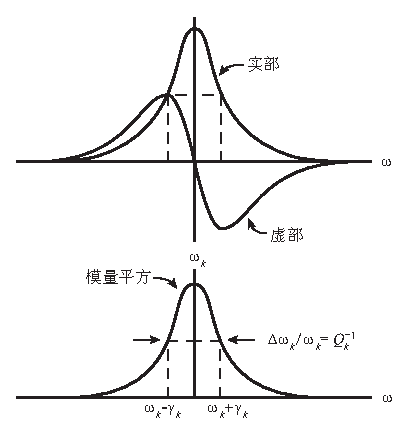
\includegraphics{../figures/chap06/fig10.eps}
\end{center}
\caption[Lorentzian]{
({\em 上\/})单位洛伦兹共振谱峰~$\eta_k(\omega)
=\textstyle{\frac{1}{2}}[\gamma_k+i(\omega-\omega_k)]^{-1}$~的实部和虚部。({\em 下\/})单位功率谱~$|\eta_k(\omega)|^2$。
}
\end{figure}
当~$Q_k \gg 1$~时,正、负峰几乎没有重叠,因此对于正频率~$\omega > 0$,(\ref{6.accFTresp})~式可以很好地近似为
\eq
\label{6.accFTresp2}
\ba(\bx,\omega)=\sum_k\bM\!:\!\overline{\beps}_k(\bx_{\rm s})
\bs_k(\bx)\eta_k(\omega),
\en
其中
\eq
\label{6.unitLor}
\eta_k(\omega)=\half[\gamma_k+i(\omega-\omega_k)]^{-1}.
\en
图~6.10~展示了{\em 单位洛伦兹谱峰\/}~$\eta_k(\omega)$~的特征形状。
\index{Lorentzian}%
相应的单位功率谱~$|\eta_k(\omega)|^2$~的最大值位于~$\omega=\omega_k$,半功率点为~$\omega=\omega_k\pm\gamma_k$。因此,每个共振峰在其半功率点处的宽度~$\Delta\omega_k$~与其相应的模式品质因子~$Q_k$~之间的关系为
\eq
\label{6.Qwidth}
\Delta\omega_k/_{\!}\omega_k=Q_k^{-1}.
\en
在严格的定量研究中,最好使用其原型~(\ref{6.accFTresp}),而避免使用~(\ref{6.accFTresp2})~这一近似,因为该近似会造成每个峰的最大值位置都与~$\omega=\omega_k$~有一个量级为~$Q_k^{-2}$~的微小偏离,且半功率宽度~$\Delta\omega_k$~也与我们熟悉的结果~(\ref{6.Qwidth})~有相同量级的差别。

(\ref{6.rotdisp})--(\ref{6.accel2})~和~(\ref{6.accFTresp})--(\ref{6.unitLor})~这些公式构成了简正模式地震学{\em 正演问题\/}的完备解,即给定地球模型和位于~$\bx_{\rm s}$~的矩张量源~$\bM$,我们就可以用它们来计算在一个地震台站~$\bx$~处的时间域或频率域的长周期响应。时间域加速度~$\ba(\bx,t)$~是衰减的正弦和余弦波的加权叠加,而其相应的频率域响应~$\ba(\bx,\omega)$~则是因耗散而变宽的共振谱峰的加权求和。每个模式的权重或复数激发振幅依赖于震源的大小和方向性~$\bM$~及其位置~$\bx_{\rm s}$。只要简单地拿掉对偶应变的上横线:$\overline{\beps}_k=\beps_k$,本节的所有结果皆适用于无自转非弹性地球。
\index{response!moment-tensor|)}%
\index{moment-tensor response|)}%
\index{hydrostatic Earth!anelastic|)}%
\index{Earth model!hydrostatic|)}%
